\videotitle{Introduction to Bayesian Optimization}
    
%-----------------------------------------------------------------------
\myframetop{Global Blackbox Optimization for Hyperparameter Optimization}{
  
    \myit{
        \item Consider the \alert{global optimization problem} of finding: 
        \[\conf^* \in \argmin_{\conf \in \confs} f(\conf)\]
        
\pause
        \item In the most general form, function $f$ is a \alert{blackbox function}:
    	\begin{center}
\scalebox{0.5}{\newcommand{\myblackbox}{\fcolorbox{black}{black}{
    \minipage[t]{\dimexpr0.111\linewidth-2\fboxsep-2\fboxrule\relax}
        ~~~\\
        ~~~\\
        ~~~\\
    \endminipage}}
    
    
    	\begin{tikzpicture}
\tikzstyle{every node}=[draw,fill=white,minimum width=0cm,thin]
\tikzstyle{every path}=[-latex,ultra thick]
\node (A) [draw=white]{{\Huge{$\conf$}}};
\node (B) [right=14mm of A,draw=white] {\myblackbox{}};
\node (C) [right=14mm of B,draw=white] {{\Huge{$f(\conf)$}}};
%\node (D) [below=7mm of B, align=center, fill=black!10] {\large{Bayesian}\\\large{optimization}};

\draw ($(A.east)+(0.2,0.0)$) -- ($(B.west)+(-0.2,0.0)$);
\draw ($(B.east)+(0.2,0.0)$) -- ($(C.west)+(-0.2,0.0)$);
%\draw ($(C.south)+(0.0,-0.2)$) -| ++(0.0,0.0) |- ($(D.east)+(0.2,0.0)$);
%\draw ($(D.west)+(-0.2,0.0)$) |- ++(0.0,0.0) -| ($(A.south)+(0.0,-0.2)$);
\end{tikzpicture}
}
    	\end{center}
    	\myit{
    		\item Only mode of interaction with $f$: querying $f$'s value at a given $\conf$ 
            \item Function $f$ may not be available in closed form, not differentiable, noisy, etc. 
    	}   
\medskip
\pause

        \item Today, we'll discuss a \alert{Bayesian} approach for solving such blackbox optimization problems
\medskip
\pause
        \item Blackbox optimization can be used for hyperparameter optimization (HPO)
        \myit{
            \item Define \alert{$f(\conf) := \mathcal{L}( \mathcal{A}_{\conf}, \mathcal{D}_{train}, \mathcal{D}_{valid} )$}
    \pause
            \item Note: for formulations of HPO that go beyond blackbox optimization, see next lecture
        }
    }
}

%----------------------------------------------------------------------
%\begin{frame}[c]{Optimization problem example}

%We know that:
%\begin{itemize}
%    \item The function $\cost$ is Lipschitz continuous and differentiable.
%    \pause
%    \item The minimizer of $\cost$ is in the interval [0,1].
%    \pause
%    \item We have observed 3 evaluations of $\cost$.
%\end{itemize}

%\end{frame}
%----------------------------------------------------------------------
%\begin{frame}[c]{Problem description}
%\framesubtitle{We have 4 function evaluations}
%\begin{figure}
%    \centering
%    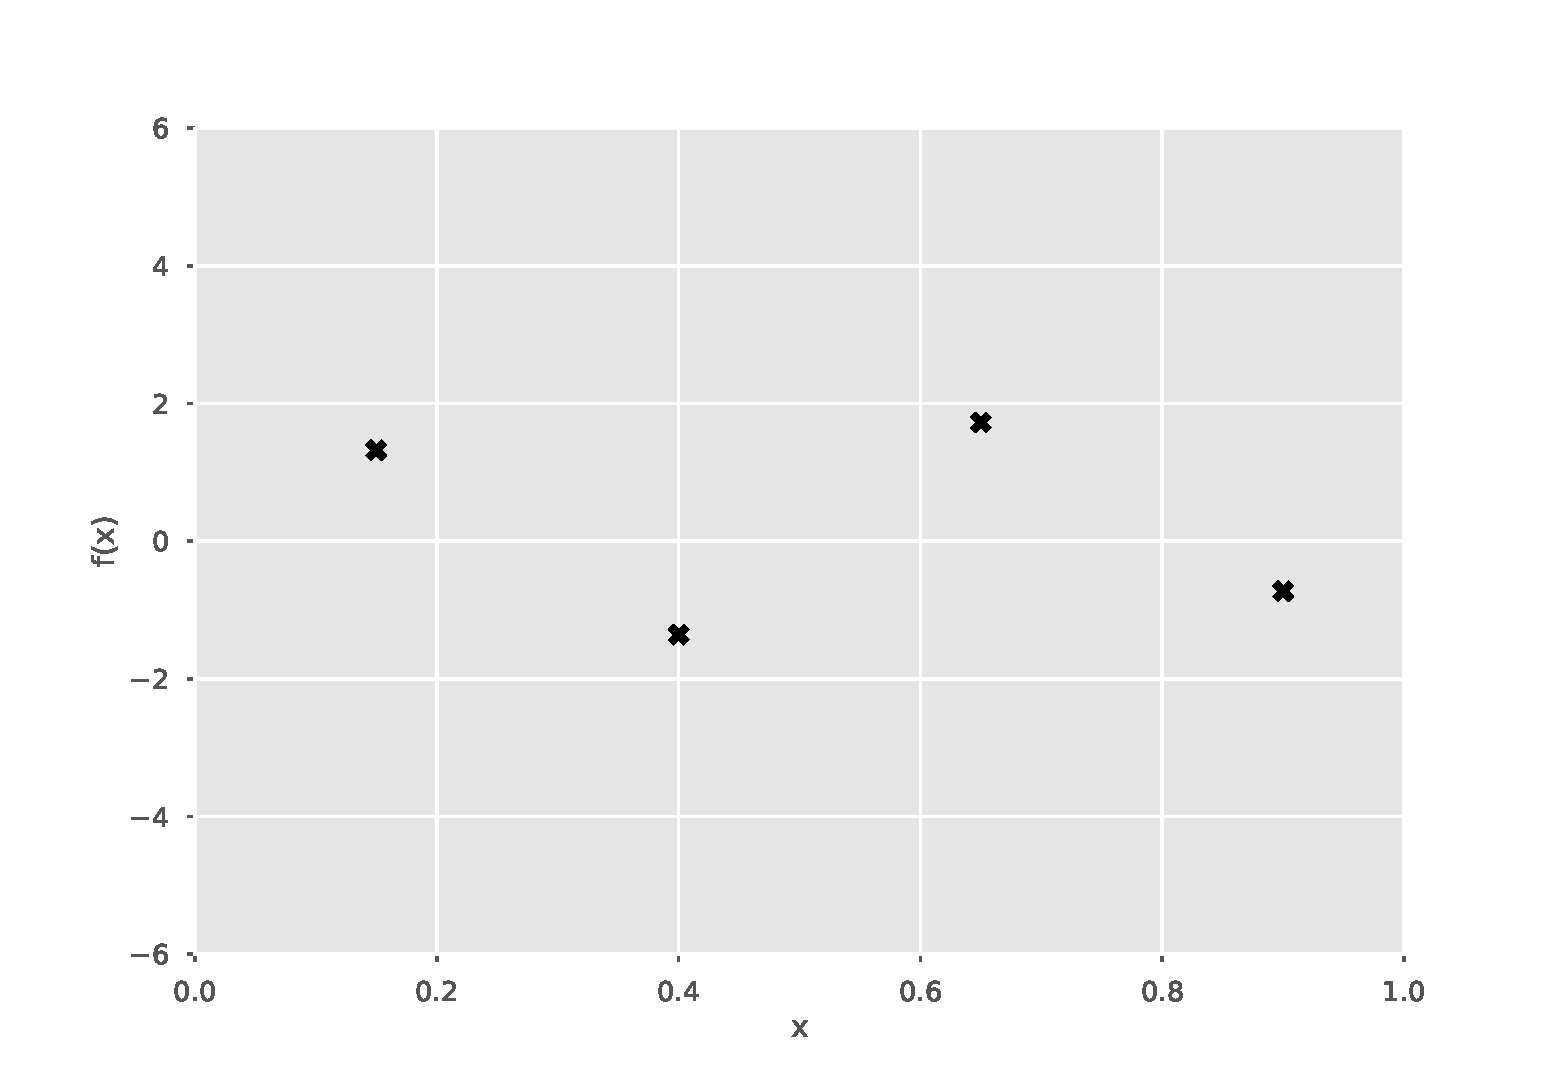
\includegraphics[width=0.8\textwidth, %height=0.38\textwidth]{images/intro_images/plot_datapoints.p%df}
%    \label{fig:my_label}
%\end{figure}
%\begin{center}
%  Where is the minimum of function $f$?  
%\end{center}
%\source{Plots are based on Javier Gonz\'alez's BO lecture %(bo\_intro.py)}



%\end{frame}

%-----------------------------------------------------------------------
%----------------------------------------------------------------------
%\begin{frame}[c]{Problem description}
%\framesubtitle{One possible curve}
%\begin{figure}
%    \centering
%    \includegraphics[width=0.7\textwidth, %height=0.4\textwidth]{images/intro_images/plot_posterior_1_s%ample.pdf}
%    \label{fig:my_label}
%\end{figure}
%\source{Plots are based on Javier Gonz\'alez's BO lecture %(bo\_intro.py)}



%\end{frame}

%-----------------------------------------------------------------------
%----------------------------------------------------------------------
%\begin{frame}[c]{Problem description}
%\framesubtitle{Three possible curves}
%\begin{figure}
%    \centering
%    \includegraphics[width=0.7\textwidth, %height=0.4\textwidth]{images/intro_images/plot_posterior_3_s%ample.pdf}
%    \label{fig:my_label}
%\end{figure}
%\source{Plots are based on Javier Gonz\'alez's BO lecture %(bo\_intro.py)}



%\end{frame}

%-----------------------------------------------------------------------
%----------------------------------------------------------------------
%\begin{frame}[c]{Problem description}
%\framesubtitle{Ten possible curves}
%\begin{figure}
%    \centering
%    \includegraphics[width=0.7\textwidth, %height=0.4\textwidth]{images/intro_images/plot_posterior_10_%sample.pdf}
%    \label{fig:my_label}
%\end{figure}
%\source{Plots are based on Javier Gonz\'alez's BO lecture %(bo\_intro.py)}



%\end{frame}

%-----------------------------------------------------------------------
%----------------------------------------------------------------------
%\begin{frame}[c]{Problem description}
%\framesubtitle{One hundred possible curves}
%\begin{figure}
%    \centering
%    \includegraphics[width=0.7\textwidth, %height=0.4\textwidth]{images/intro_images/plot_posterior_100%_sample.pdf}
%    \label{fig:my_label}
%\end{figure}
%\source{Plots are based on Javier Gonz\'alez's BO lecture %(bo\_intro.py)}



%\end{frame}

%-----------------------------------------------------------------------%----------------------------------------------------------------------
%\begin{frame}[c]{Problem description}
%\framesubtitle{One thousand possible curves}
%\begin{figure}
%    \centering
%    \includegraphics[width=0.7\textwidth, %height=0.4\textwidth]{images/intro_images/plot_posterior_100%0_sample.pdf}
%    \label{fig:my_label}
%\end{figure}
%\source{Plots are based on Javier Gonz\'alez's BO lecture (bo\_intro.py)}



%\end{frame}

%-----------------------------------------------------------------------
%----------------------------------------------------------------------
%\begin{frame}[c]{Problem description}
%\framesubtitle{Infinitely many curves}
%\begin{figure}
%    \centering
%    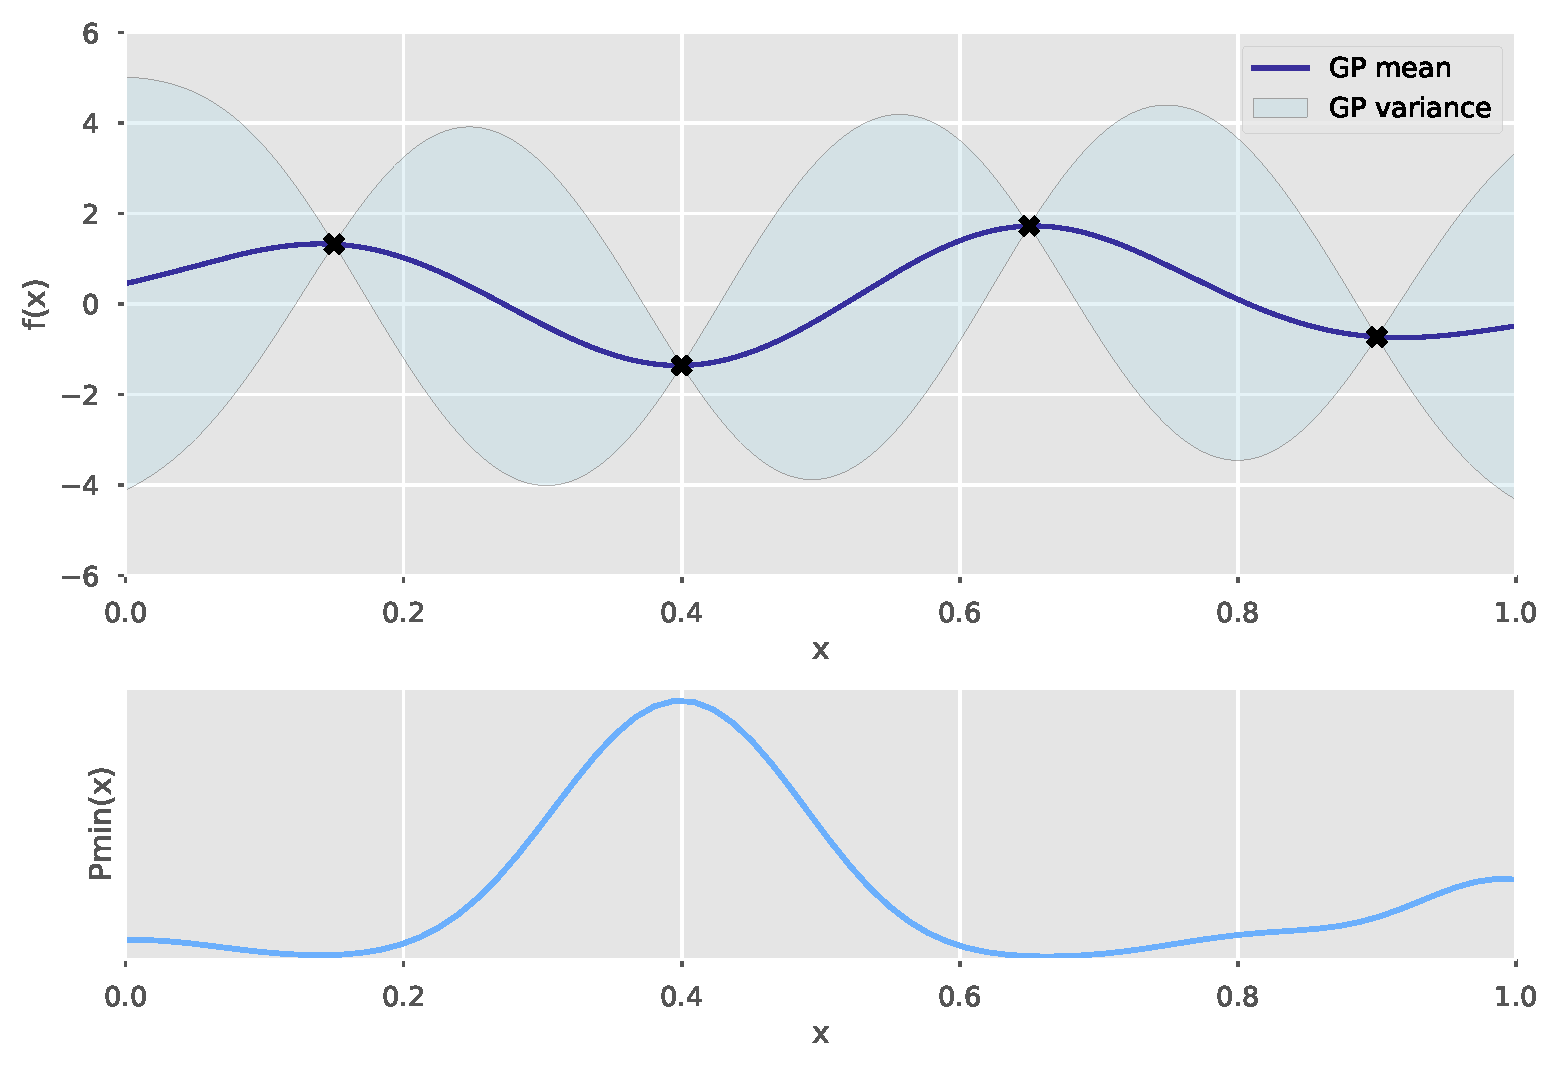
\includegraphics[width=0.7\textwidth, %height=0.4\textwidth]{images/intro_images/plot_posterior.pdf%}
%    \label{fig:my_label}
%\end{figure}
%\source{Plots are based on Javier Gonz\'alez's BO lecture (bo\_intro.py)}


%\end{frame}
%----------------------------------------------------------------------
\myframetop{Bayesian Optimization of a blackbox function in a nutshell}{

\bigskip
\bigskip
\bigskip

    \onslide<1->
    \begin{figure}
        \vspace{-1em}
        \centering
        \only<1>{
            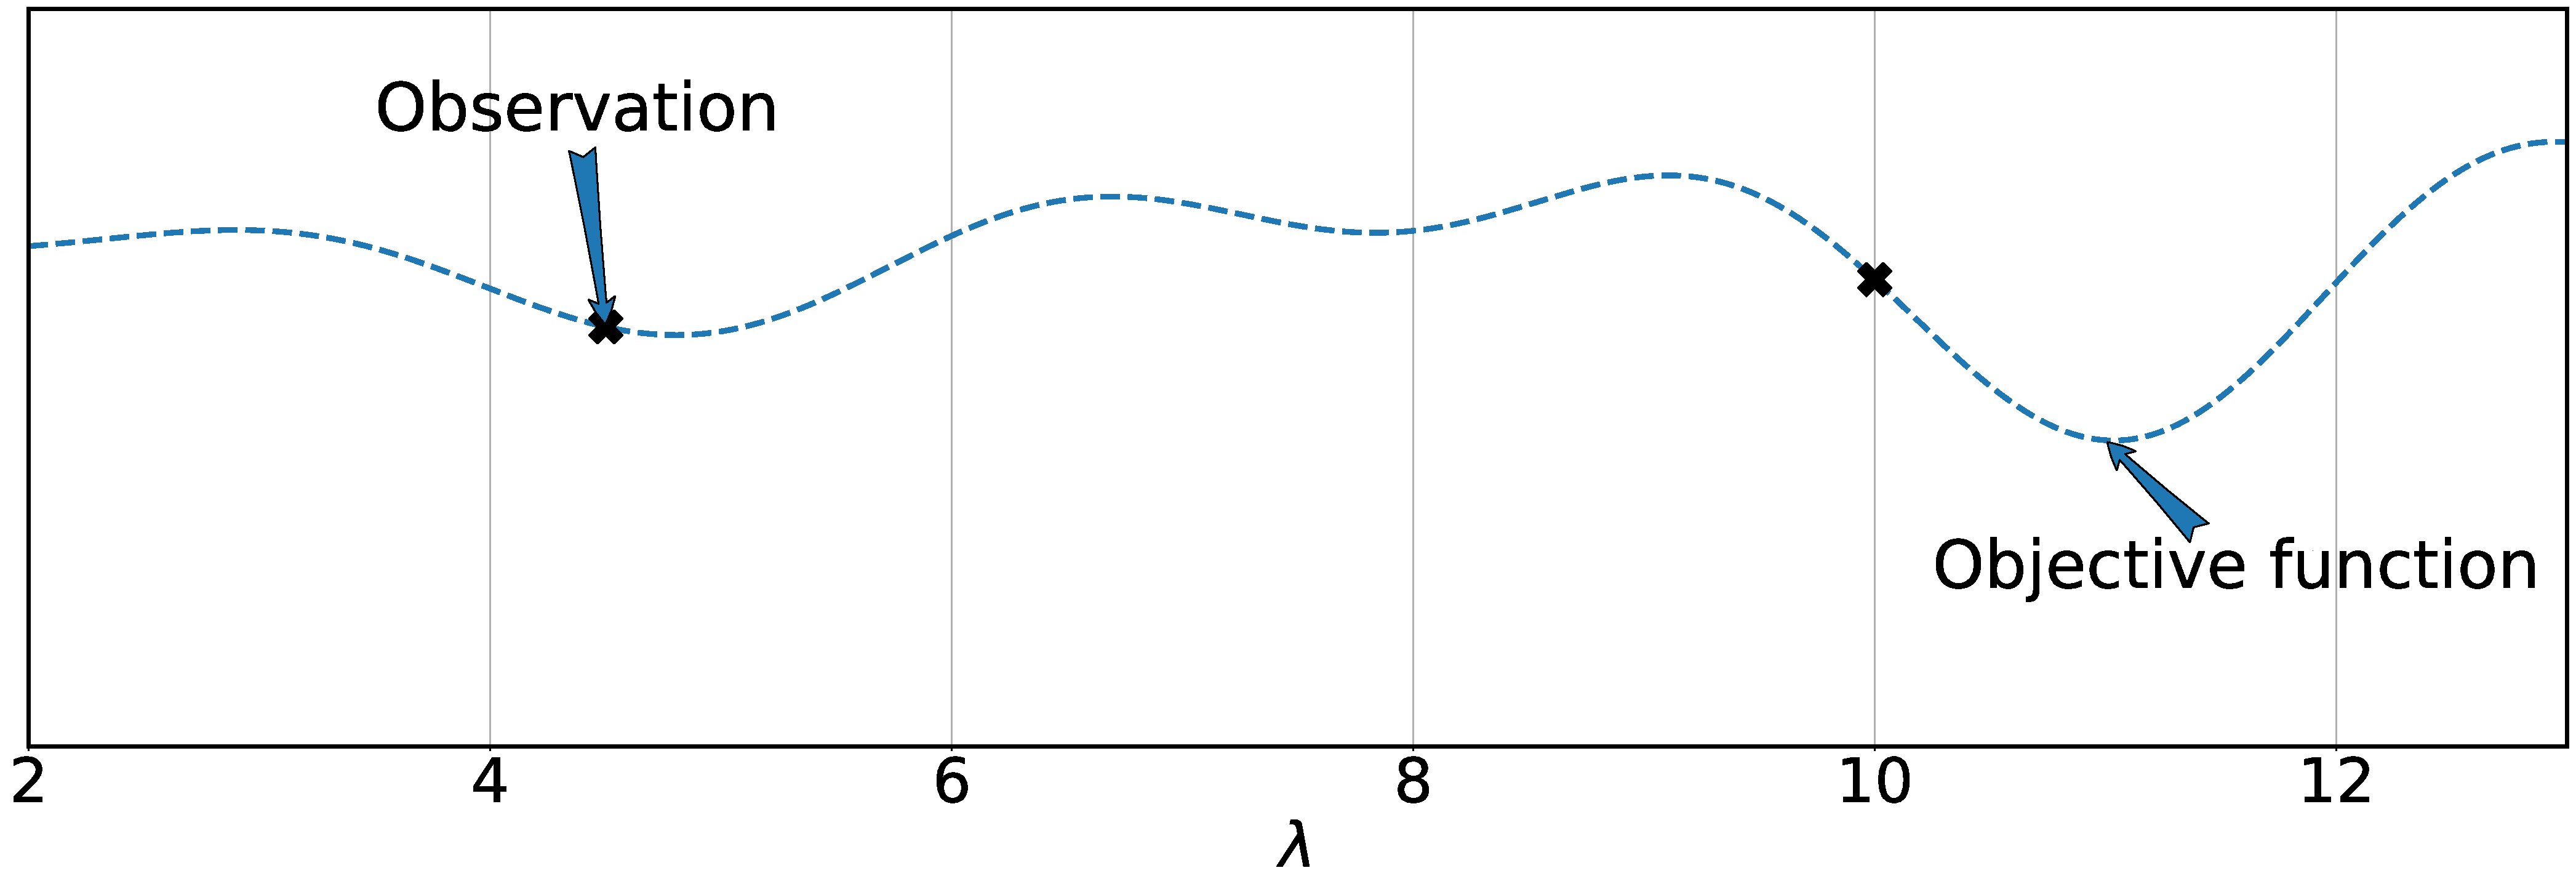
\includegraphics[width=0.95\textwidth]{images/intro_images/IntroPlots_Obs.pdf}
        }\only<2>{
            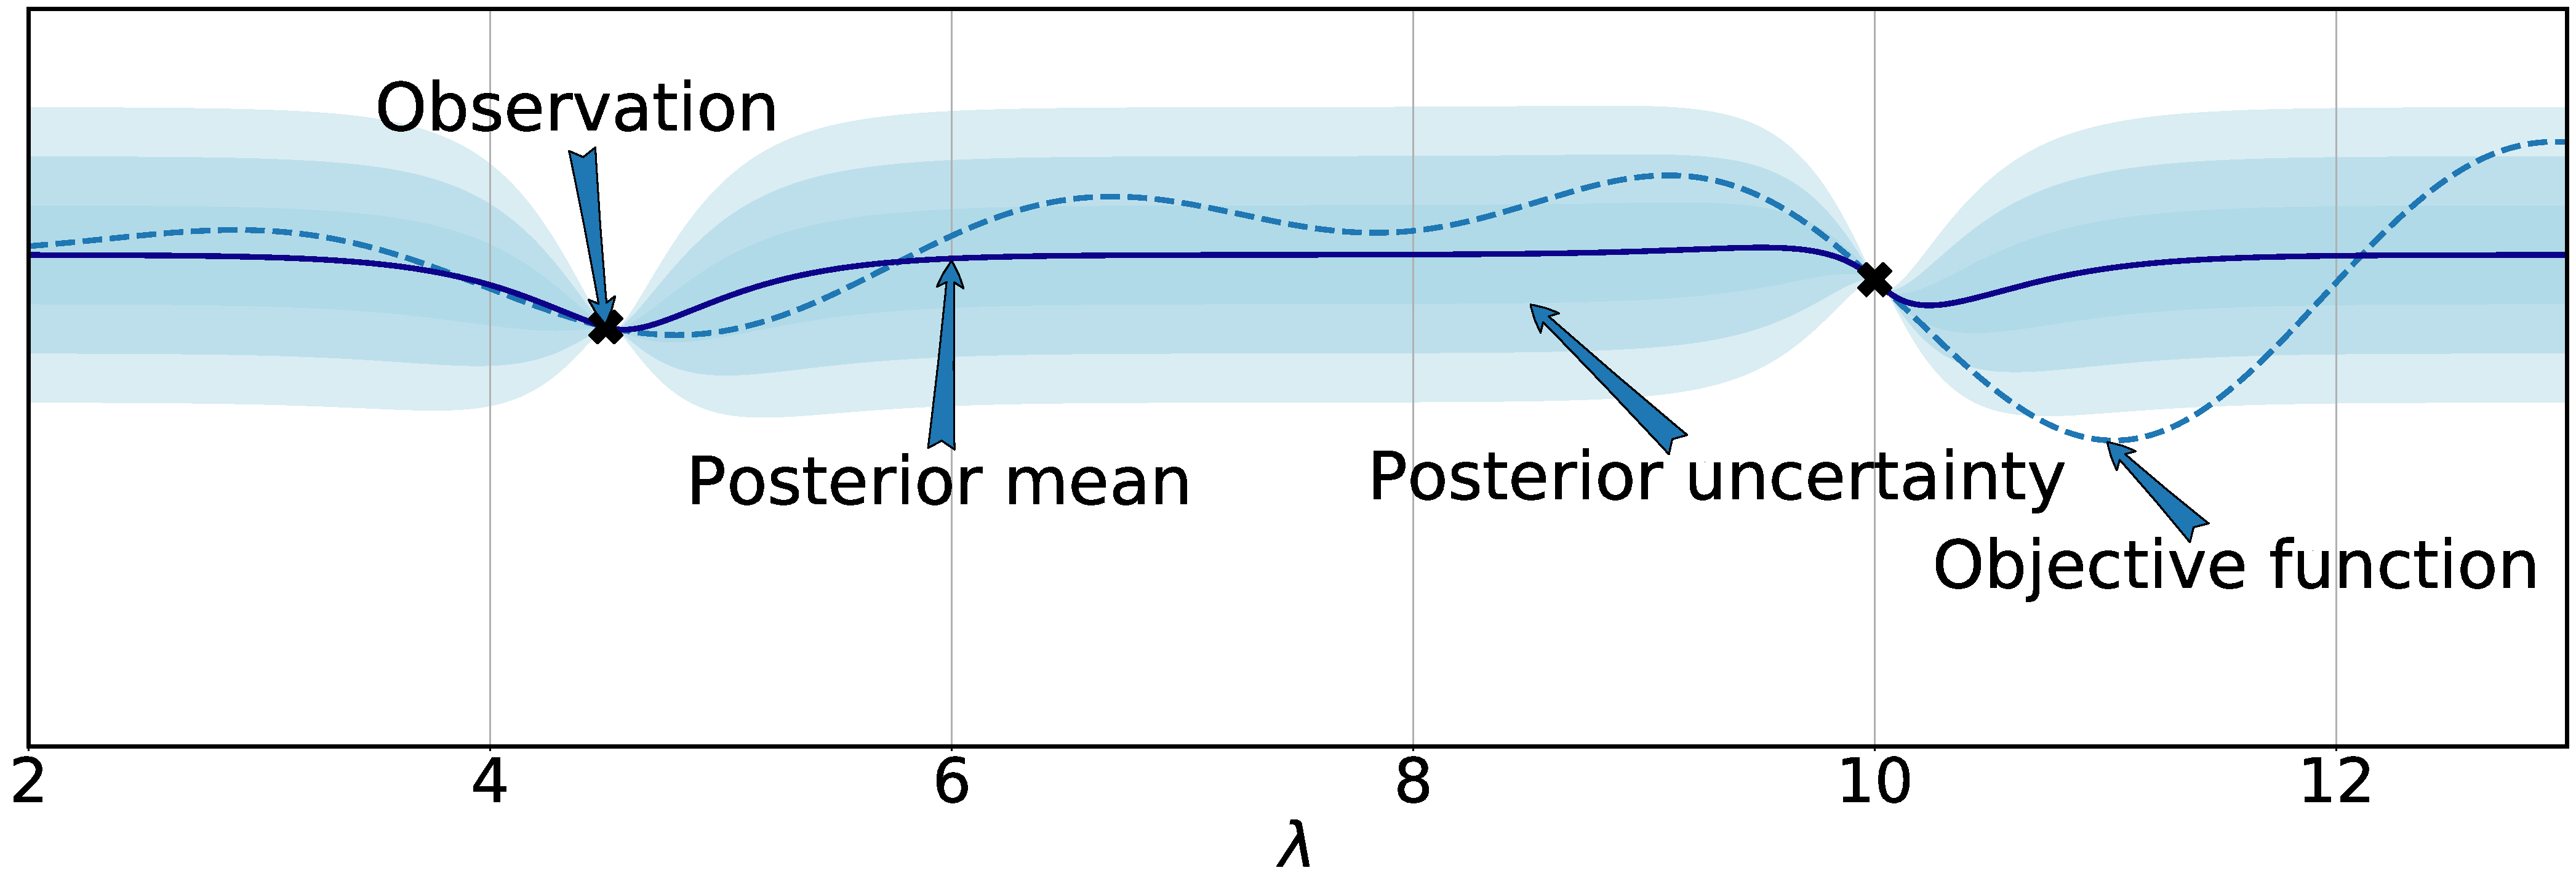
\includegraphics[width=0.95\textwidth]{images/intro_images/IntroPlots_GP.pdf}
        }\only<3>{
            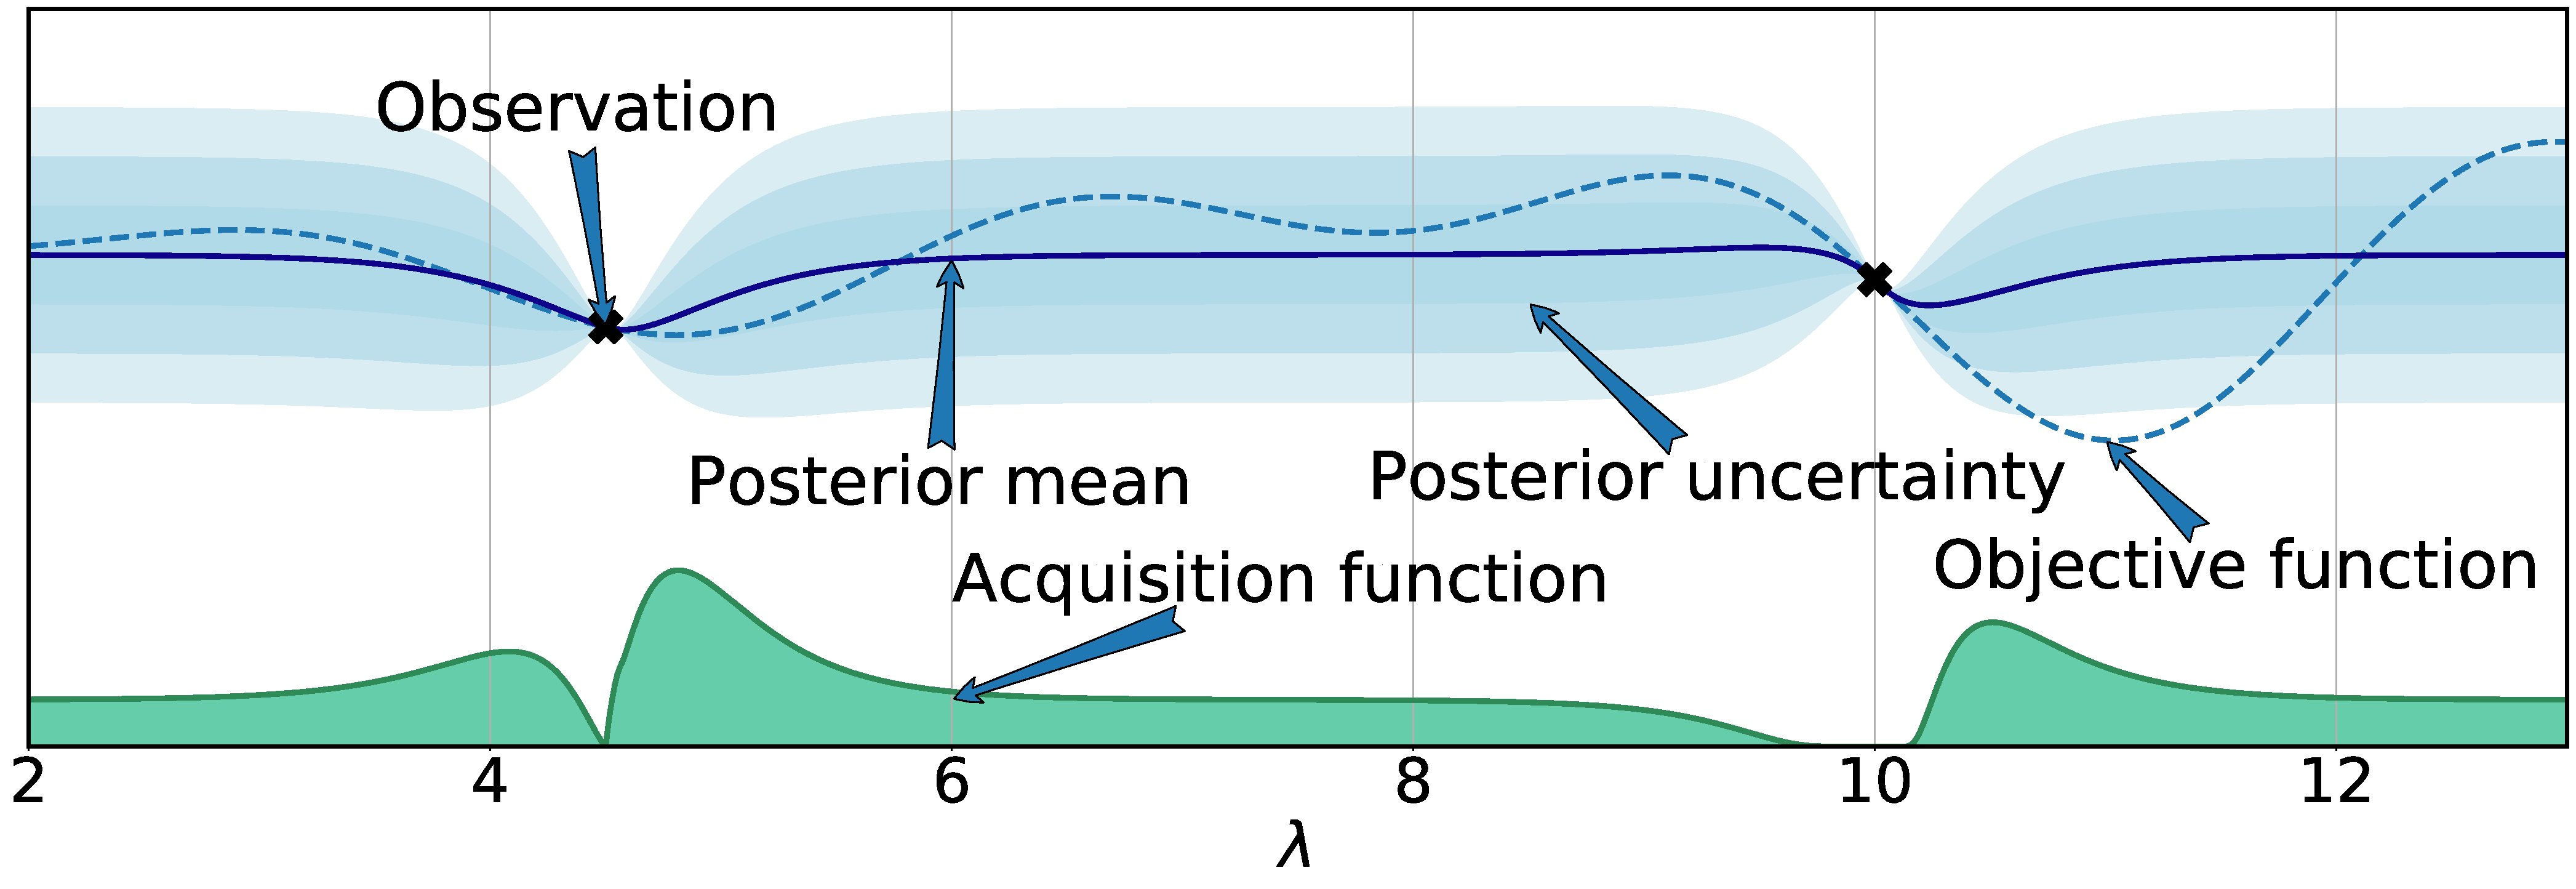
\includegraphics[width=0.95\textwidth]{images/intro_images/IntroPlots_Acqui.pdf}
        }\only<4->{
            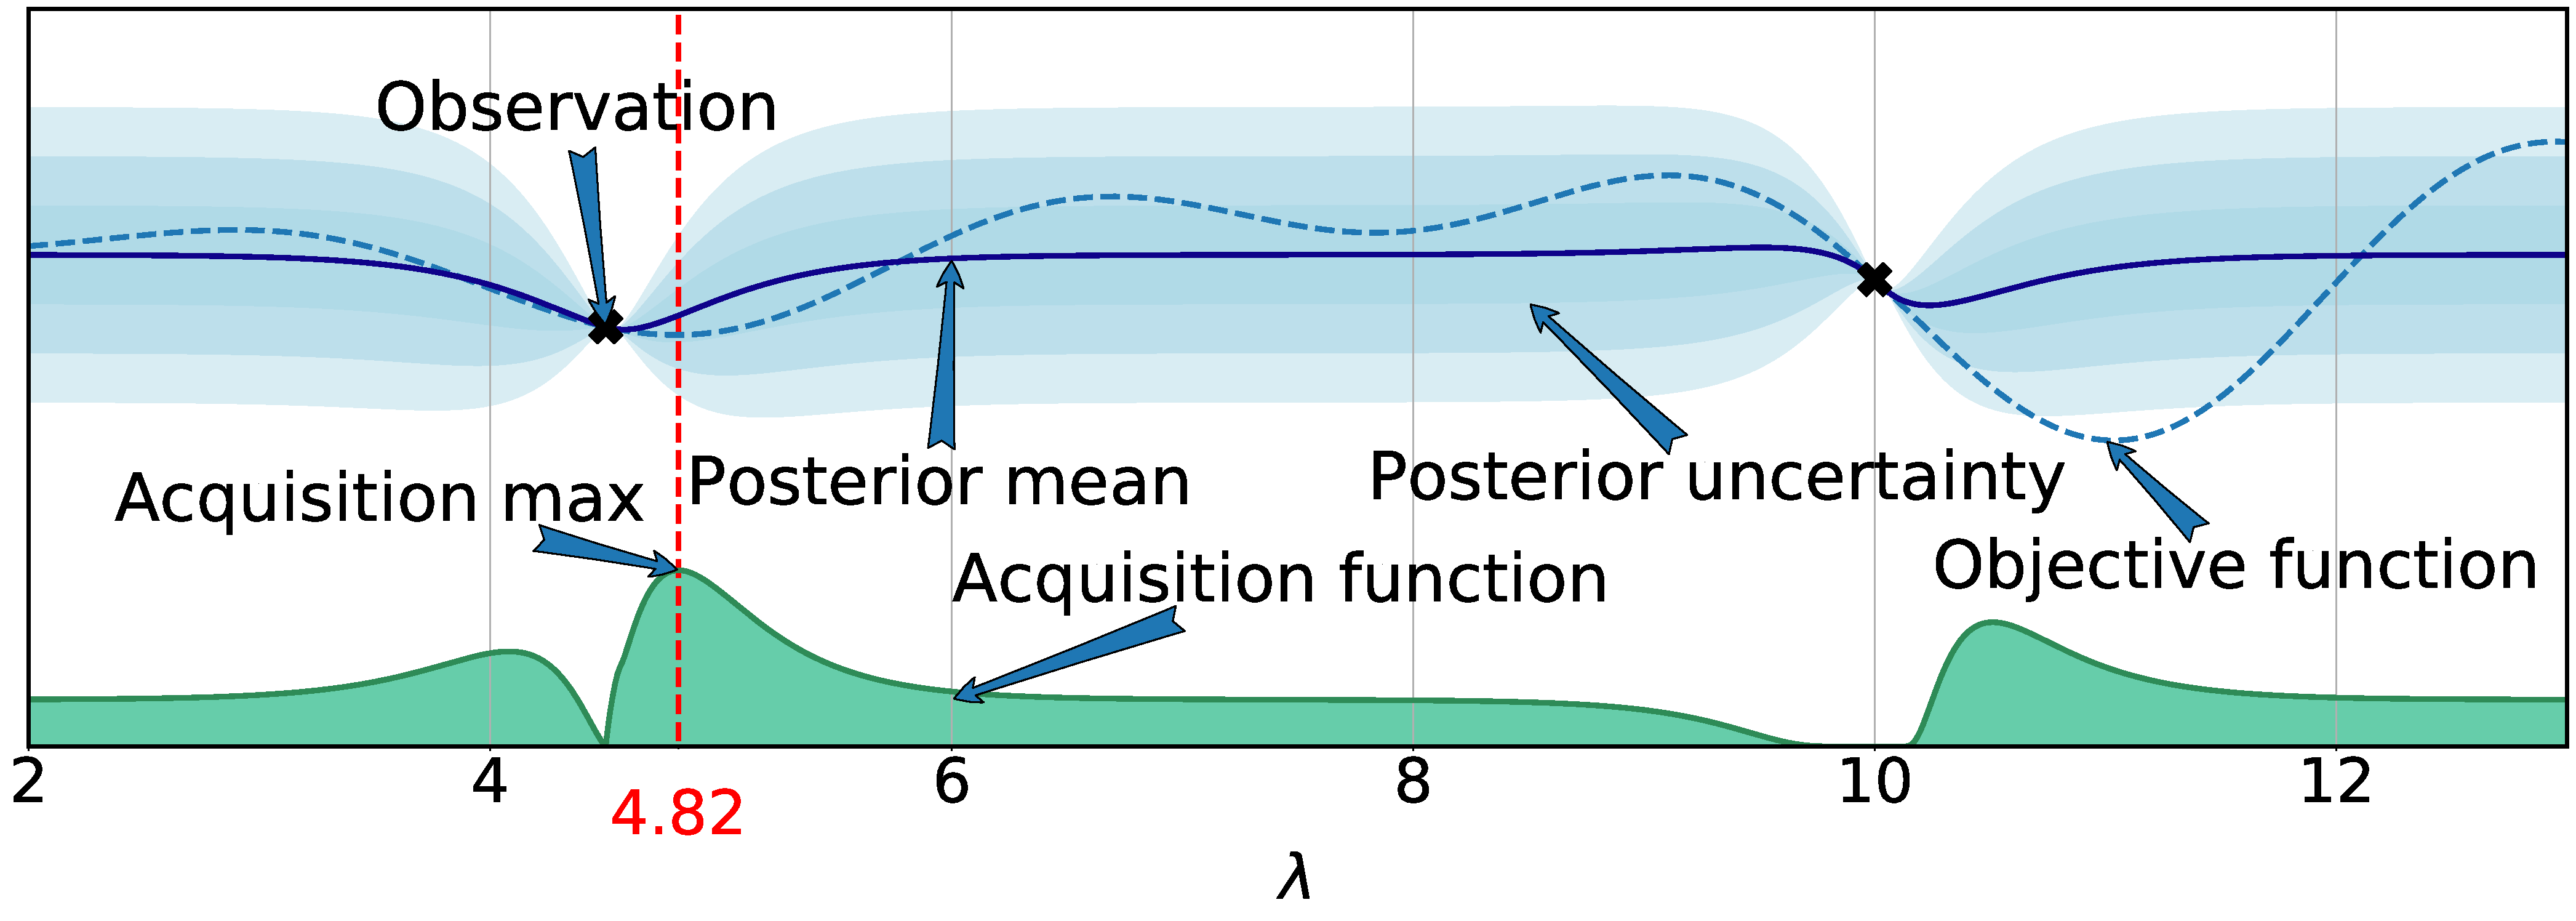
\includegraphics[width=0.95\textwidth]{images/intro_images/IntroPlots_Complete.pdf}
        }
    \end{figure}
    
% \vspace*{-0.5cm}\notefh{Can you please increase the plotted values of the acquisition function, so that it is more clearly visible? Also on the next slide. You could, e.g., normalize it to have a certain maximum (a bit larger than that of the third plot on the next slide). Also, on the next slide, can you please plot the new observation red, not green?}
}

%----------------------------------------------------------------------
\begin{frame}[c]{Bayesian Optimization of a blackbox function in a nutshell}

\begin{columns}[T]
\column{0.45\textwidth}
General approach
\begin{itemize}
    \item Fit a \alert{probabilistic model} to the collected function samples $\langle{}\conf, \cost(\conf)\rangle{}$
    \item Use the model to guide optimization, trading off \alert{exploration \vs{} exploitation}
%    \item Acquisition function for exploration-exploitation tradeoff
%    \item Optimize on acquisition function\\ to get next $x$ $\conf$ ($x$)
\end{itemize}

\bigskip

\onslide<4->{
    \alert{Popular approach in the statistics literature} since
    \href{http://link.springer.com/chapter/10.1007\%2F3-540-07165-2_55}{\footnotesize\color{black!70} Mockus et al. [1978]}
    \begin{itemize}
        \item Efficient in \#function evaluations
        \item Works when objective is \alert{nonconvex, noisy, has unknown derivatives, etc.}
        \item Recent \alert{convergence} results\\ \lit{\href{https://arxiv.org/abs/0912.3995}{Srinivas et al. 2009}; \href{http://www.jmlr.org/papers/v12/bull11a.html}{Bull et al. 2011}; \href{https://www.cs.ubc.ca/~nando/papers/BayesBandits.pdf}{de Freitas et al. 2012}; \href{http://papers.nips.cc/paper/5715-bayesian-optimization-with-exponential-convergence}{Kawaguchi et al. 2015}}
    %    \item Popular \alert{Bayesian optimization workshop} at NIPS (the premiere machine learning conference)
    \end{itemize}
}

\column{0.55\textwidth}
\onslide<1->
\begin{figure}
    \vspace{-1em}
    \centering
    \onslide<1->{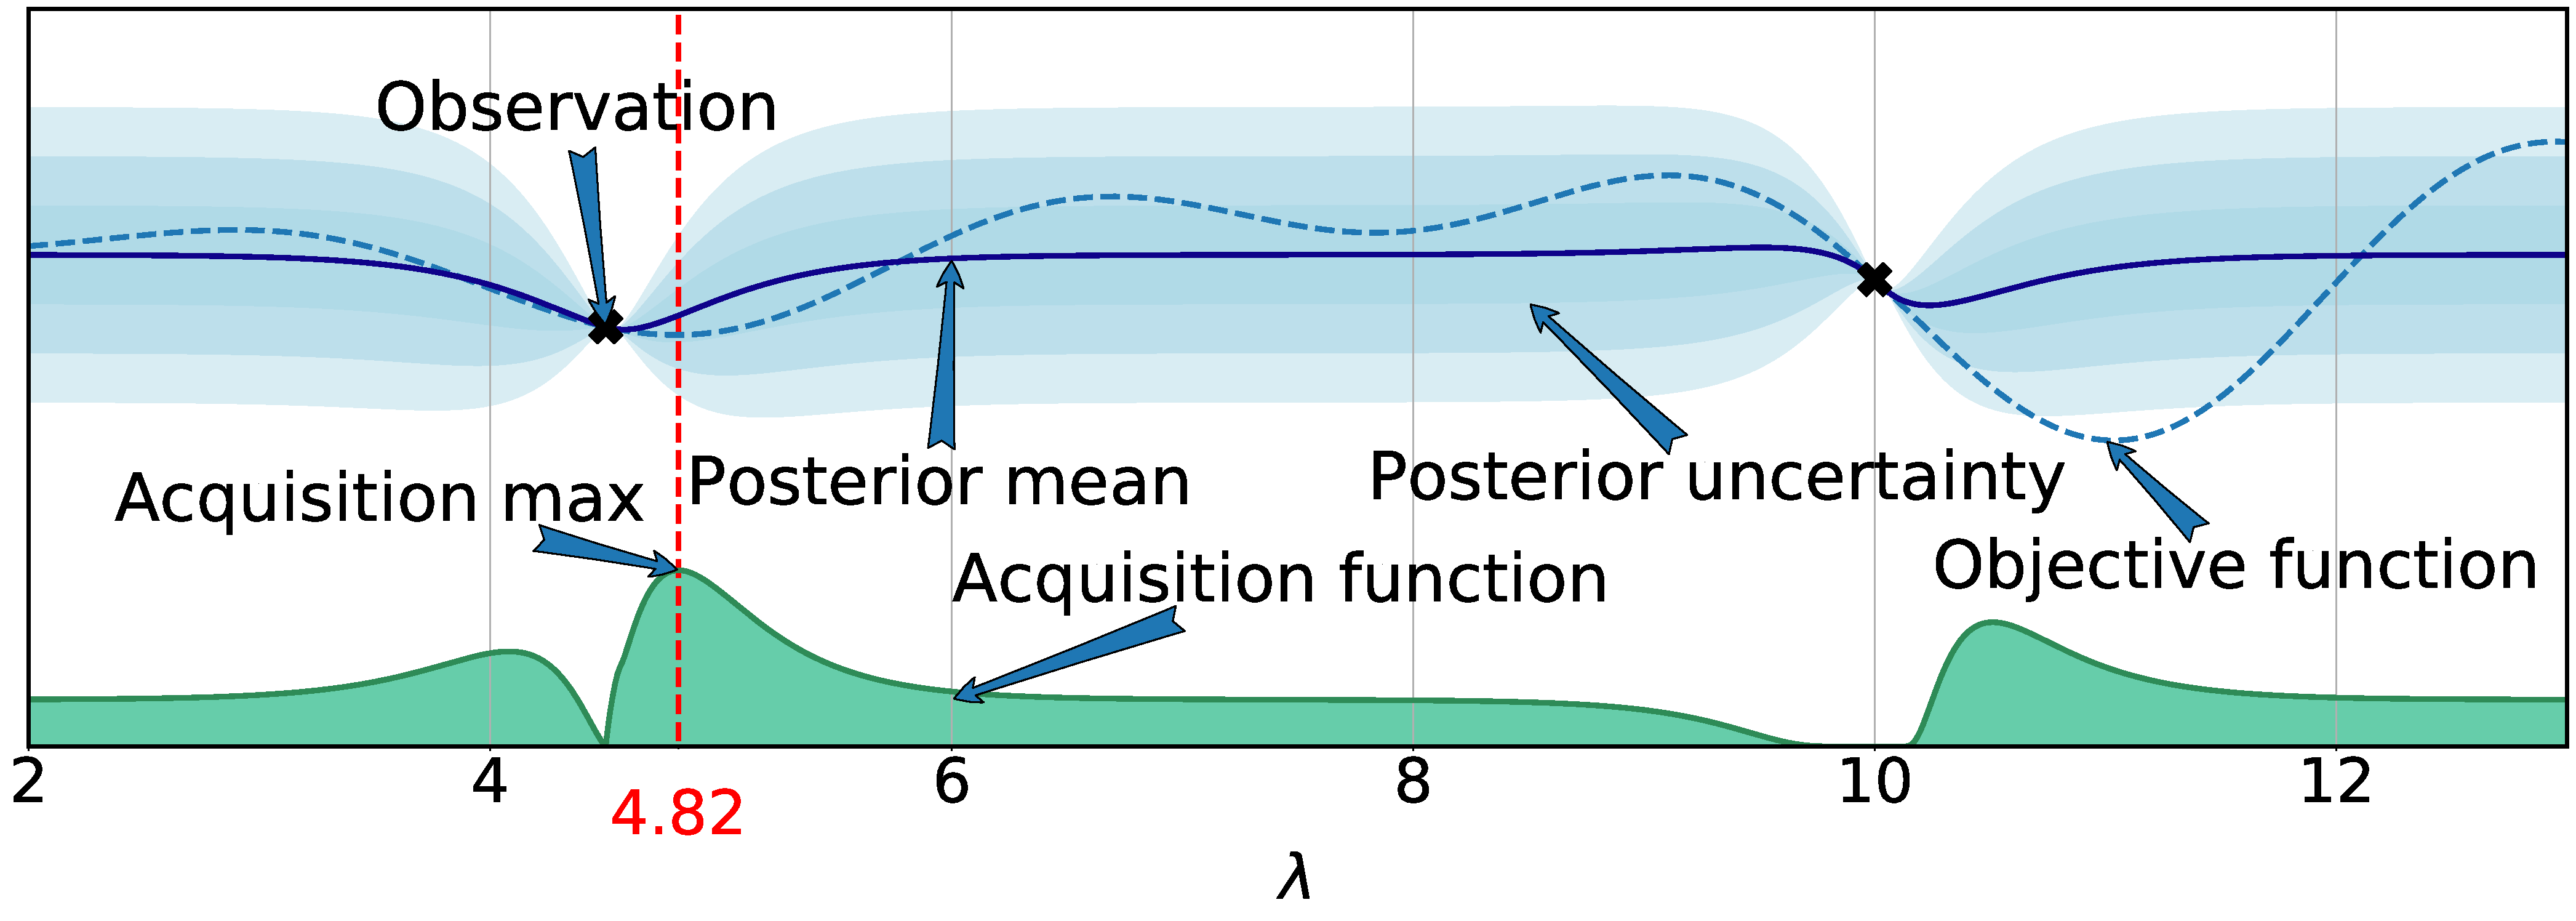
\includegraphics[width=0.8\textwidth]{images/intro_images/IntroPlots_Iter2.pdf}}
    \onslide<2->{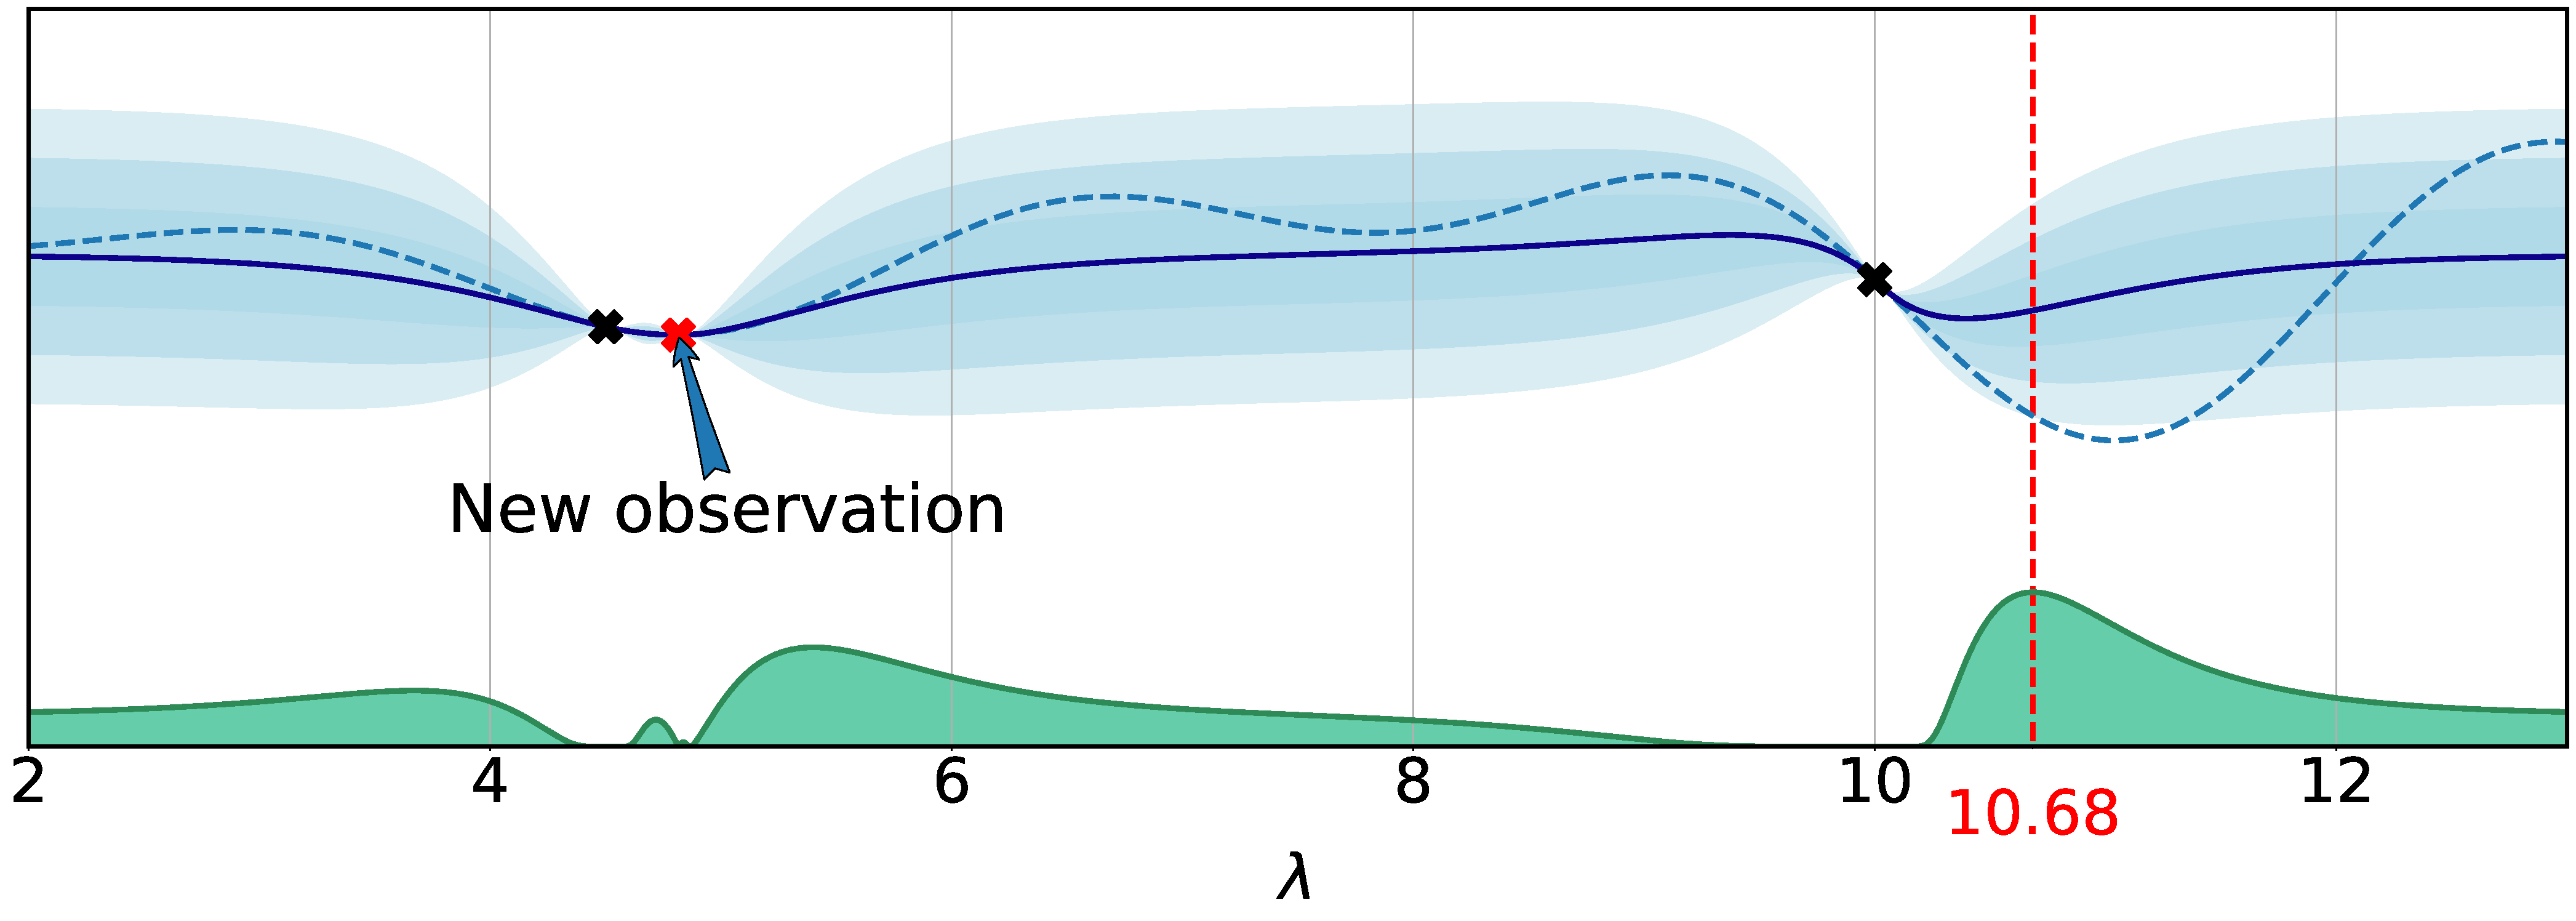
\includegraphics[width=0.8\textwidth]{images/intro_images/IntroPlots_Iter3.pdf}}
    \onslide<3->{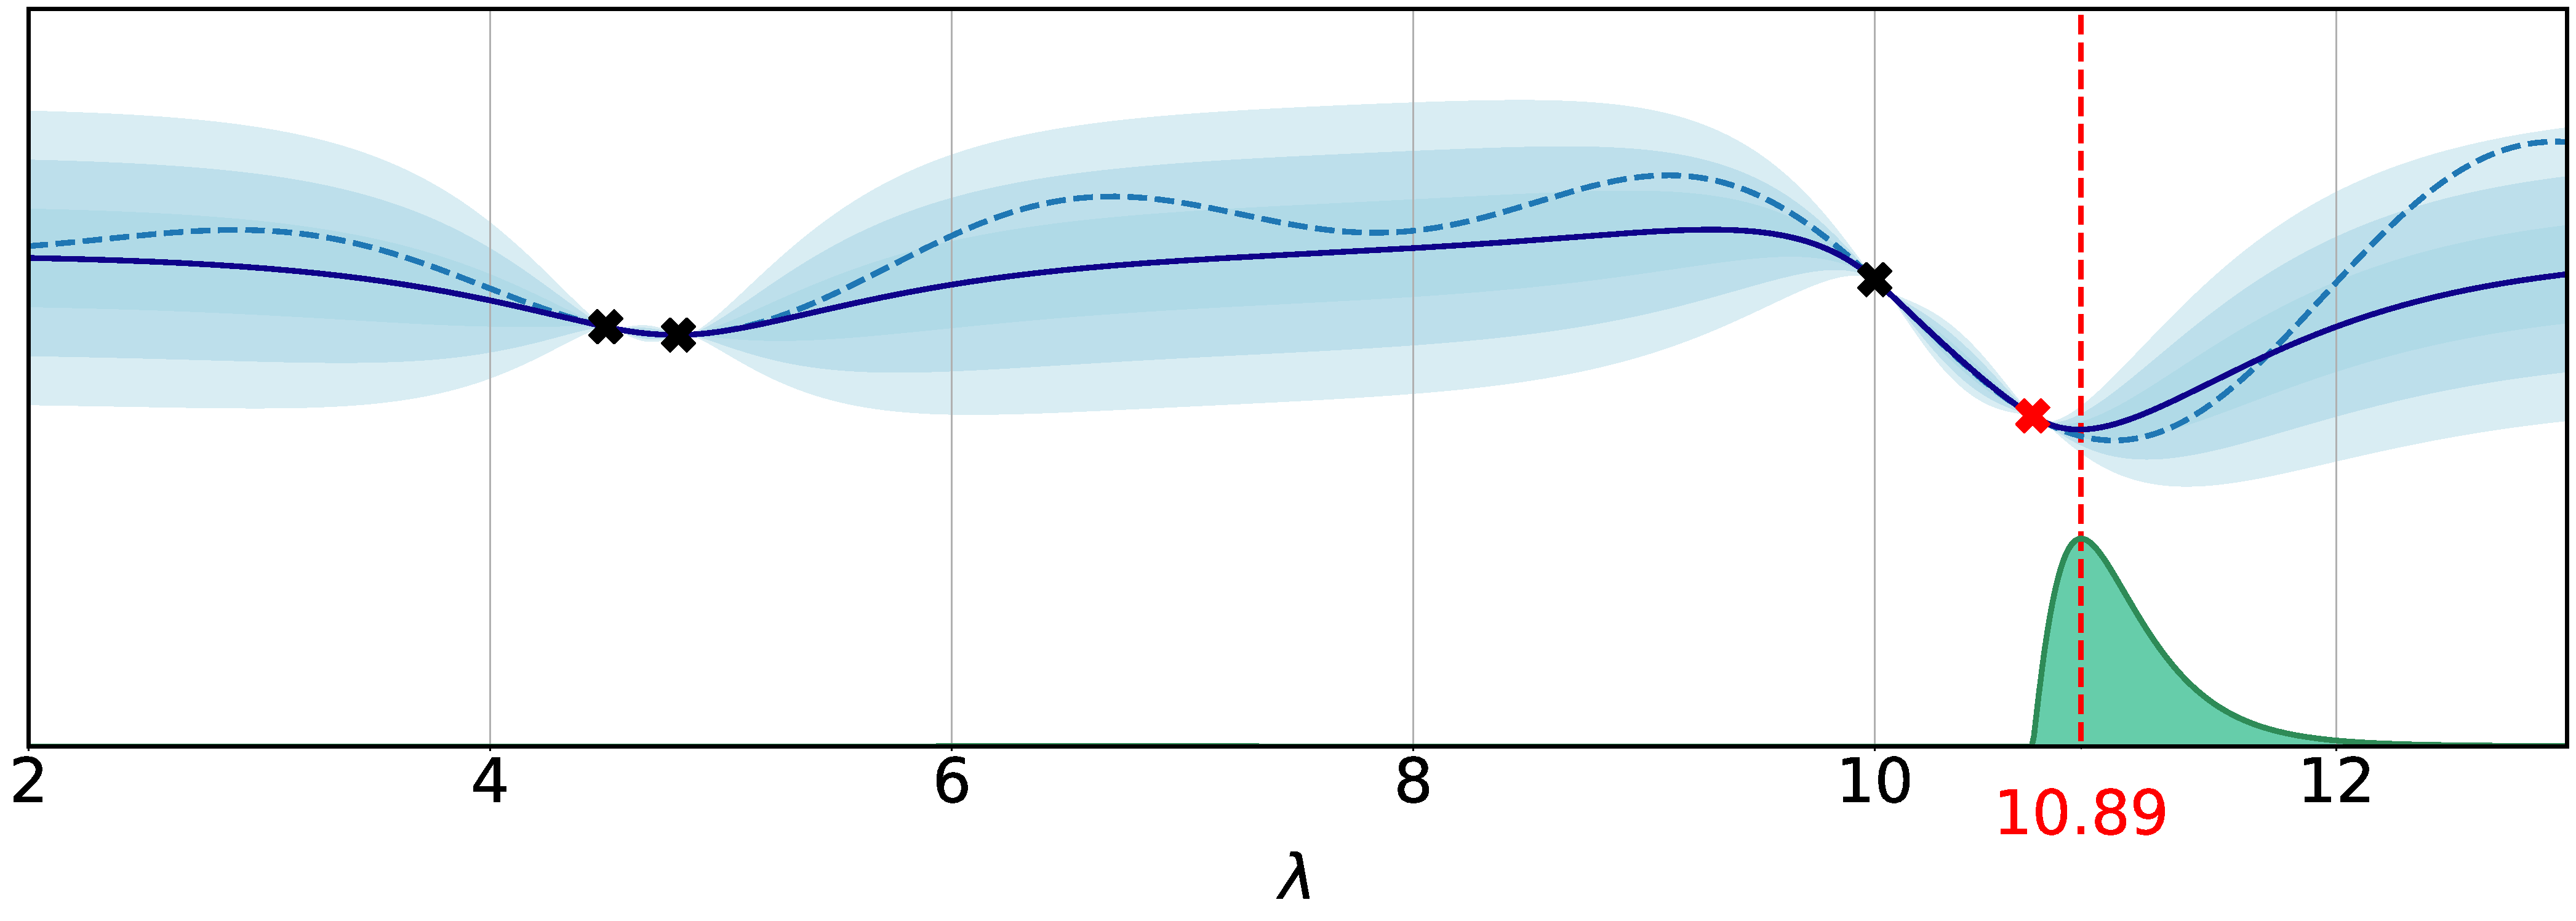
\includegraphics[width=0.8\textwidth]{images/intro_images/IntroPlots_Iter4.pdf}}
    %\only<4>{\includegraphics[width=\textwidth]{images/intro_images/plot_2.pdf}}
    %\only<5>{\includegraphics[width=\textwidth]{images/intro_images/plot_3.pdf}}
    %\only<6>{\includegraphics[width=\textwidth]{images/intro_images/plot_4.pdf}}
    %\only<7>{\includegraphics[width=\textwidth]{images/intro_images/plot_5.pdf}}
    %\only<8>{\includegraphics[width=\textwidth]{images/intro_images/plot_6.pdf}}
    %\only<9->{\includegraphics[width=\textwidth]{images/intro_images/plot_7.pdf}}
\end{figure}
\end{columns}

\end{frame}
%-----------------------------------------------------------------------
%\myframe{Bayesian Optimization in a Nutshell}{
%  
%\vspace*{-0.5cm}
%\begin{columns}[T]
%
%\column{0.6\textwidth}
%
%\myblock{General approach}{
%	\myit{
%	  \item Fit a probabilistic model to the collected function samples
%	  $\langle{}\conf, \cost(\conf)\rangle{}$
%	  \item Use the model to guide optimization, trading off
%	  exploration \vs{} exploitation
%	%  \item Acquisition function for exploration-exploitation tradeoff
%	%  \item Optimize on acquisition function\\ to get next $x$
%	  %$\conf$ ($x$)
%	}
%}
%
%\smallskip
%\onslide<5->{
%	\myblock{Popular approach in the statistics literature since \litw{\href{http://link.springer.com/chapter/10.1007\%2F3-540-07165-2_55}{Mockus,
%	1978}}}{ \myit{
%		  	\item Efficient in \# function evaluations 
%		  	\item Works when objective is nonconvex, noisy, has unknown derivatives, etc
%			\pause
%			\item Recent convergence results\\ \lit{Srinivas et al, 2010; Bull 2011;
%			de Freitas et al, 2012; Kawaguchi et al, 2015}
%			%TODO: sorry, I don't know these papers
%		%	\item Popular \alert{Bayesian optimization workshop} at NIPS (the premiere machine learning conference)
%		}
%	}
%}
%%\begin{enumerate}
%%  \item Fit an empirical performance model (EPM) 
%%  \item Acquisition function for exploration-exploitation tradeoff
%%  \item Optimize on acquisition function\\ to get next $\conf$ ($x$)
%%\end{enumerate}
%
%\column{0.4\textwidth}
%\vspace*{0.5cm}
%\onslide<2->{
%	%\includegraphics[width=1\textwidth]{../images/bo.png}
%	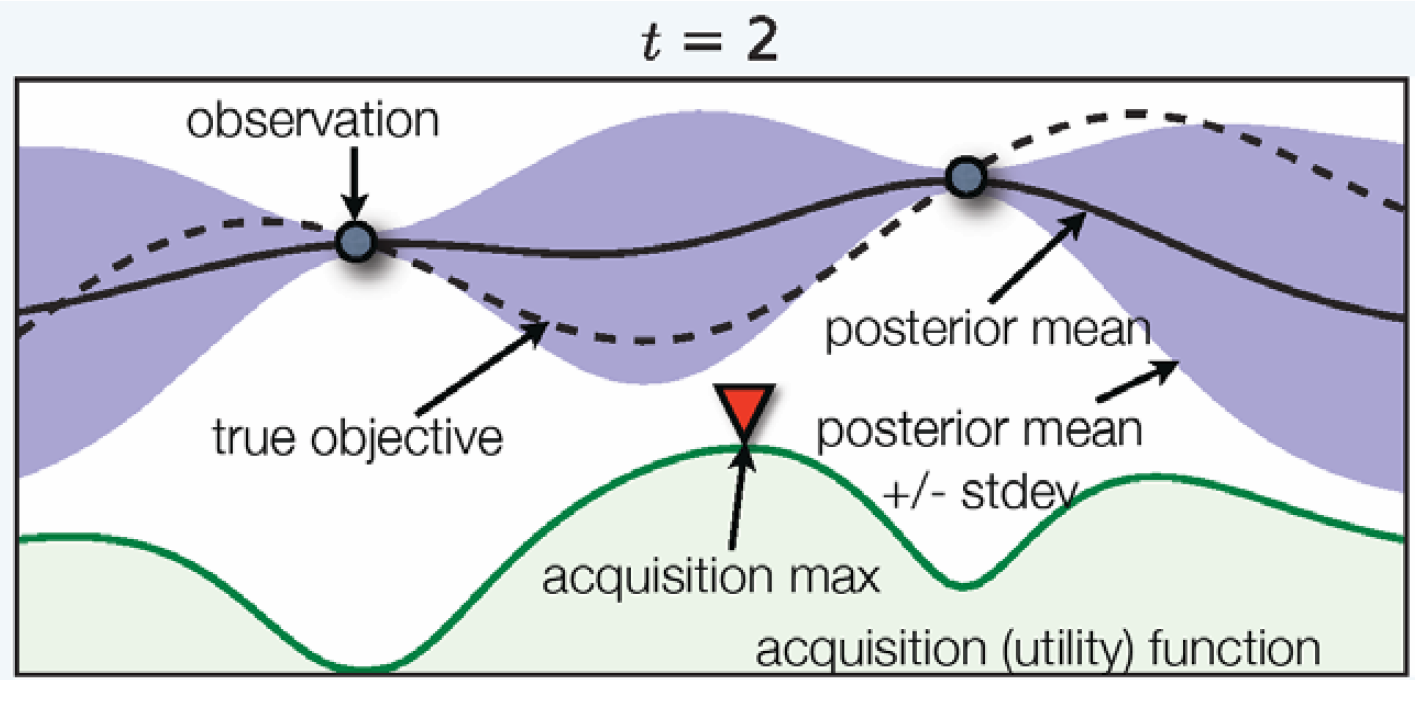
\includegraphics[width=0.9\textwidth]{plots_and_scripts/plots/bo_pic1.png}\\
%	\pause
%	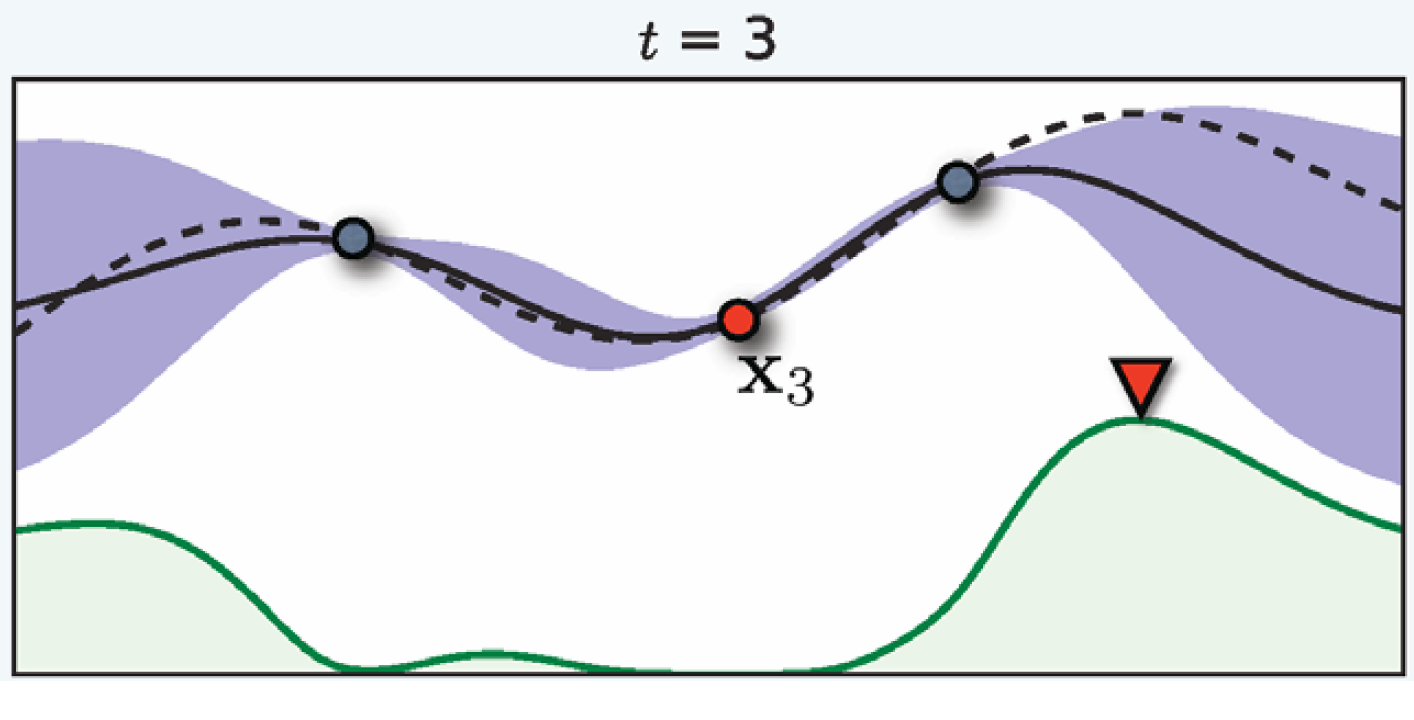
\includegraphics[width=0.9\textwidth]{plots_and_scripts/plots//bo_pic2.png}\\
%	\pause
%	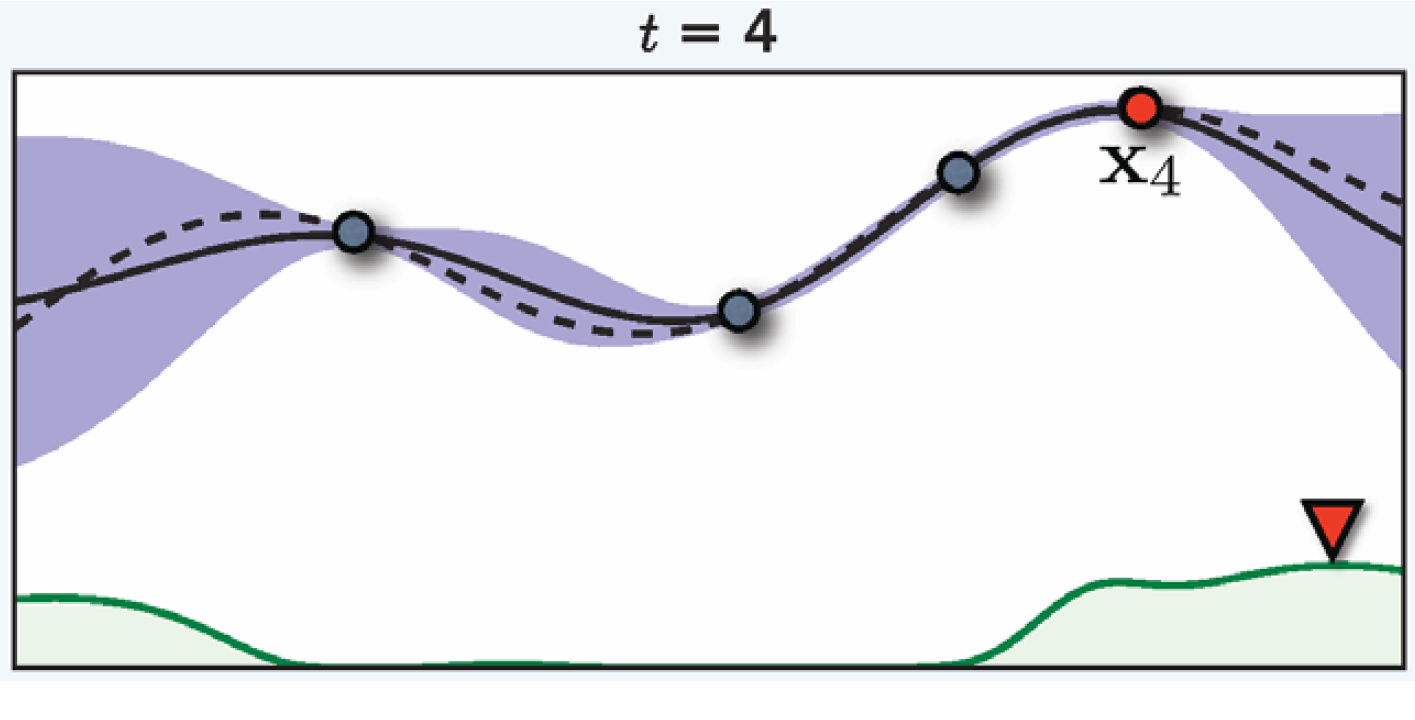
\includegraphics[width=0.9\textwidth]{plots_and_scripts/plots//bo_pic3.png}\\
%	\footnotesize{Image source: \lit{\href{https://arxiv.org/abs/1012.2599}{Brochu et al, 2010}}}
%}
%\end{columns}
%}
%----------------------------------------------------------------------
%5\begin{frame}[c]{Bayesian Optimization: Visualization of Many Steps}
%\begin{figure}
%    \centering
%    \only<1>{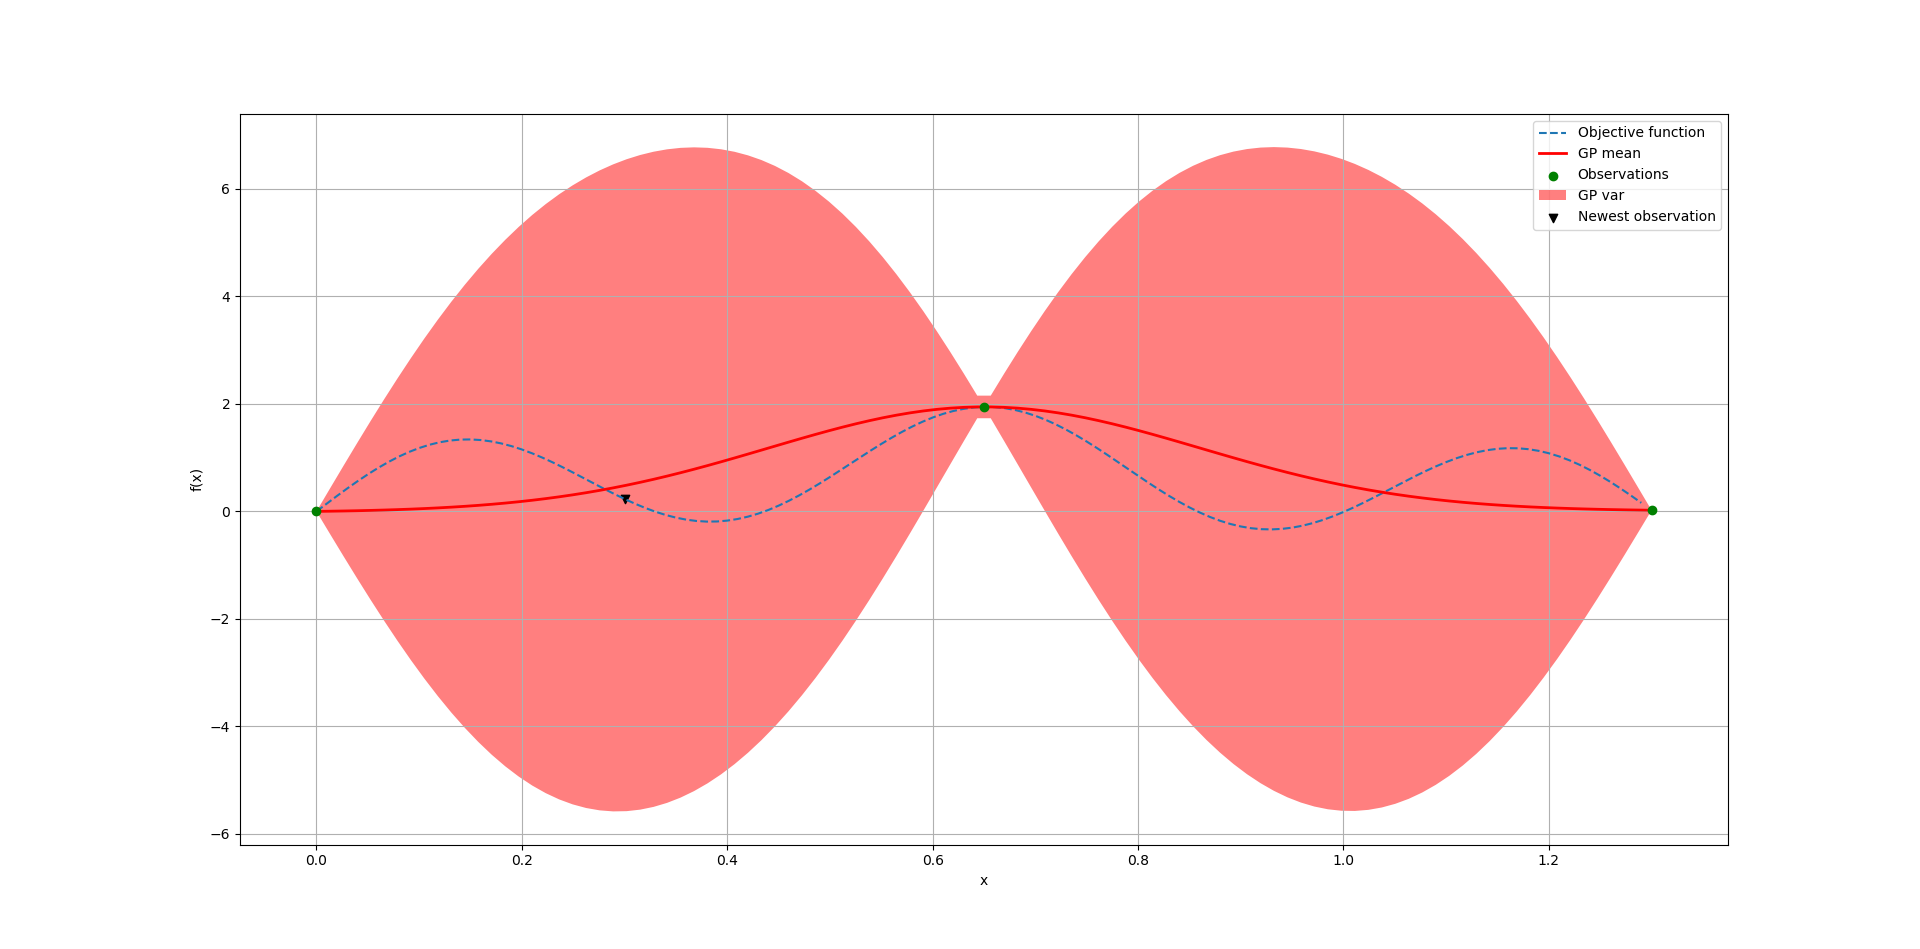
\includegraphics[width=\linewidth]{images/intro_images/BOLoop_1.png}}
%    \only<2>{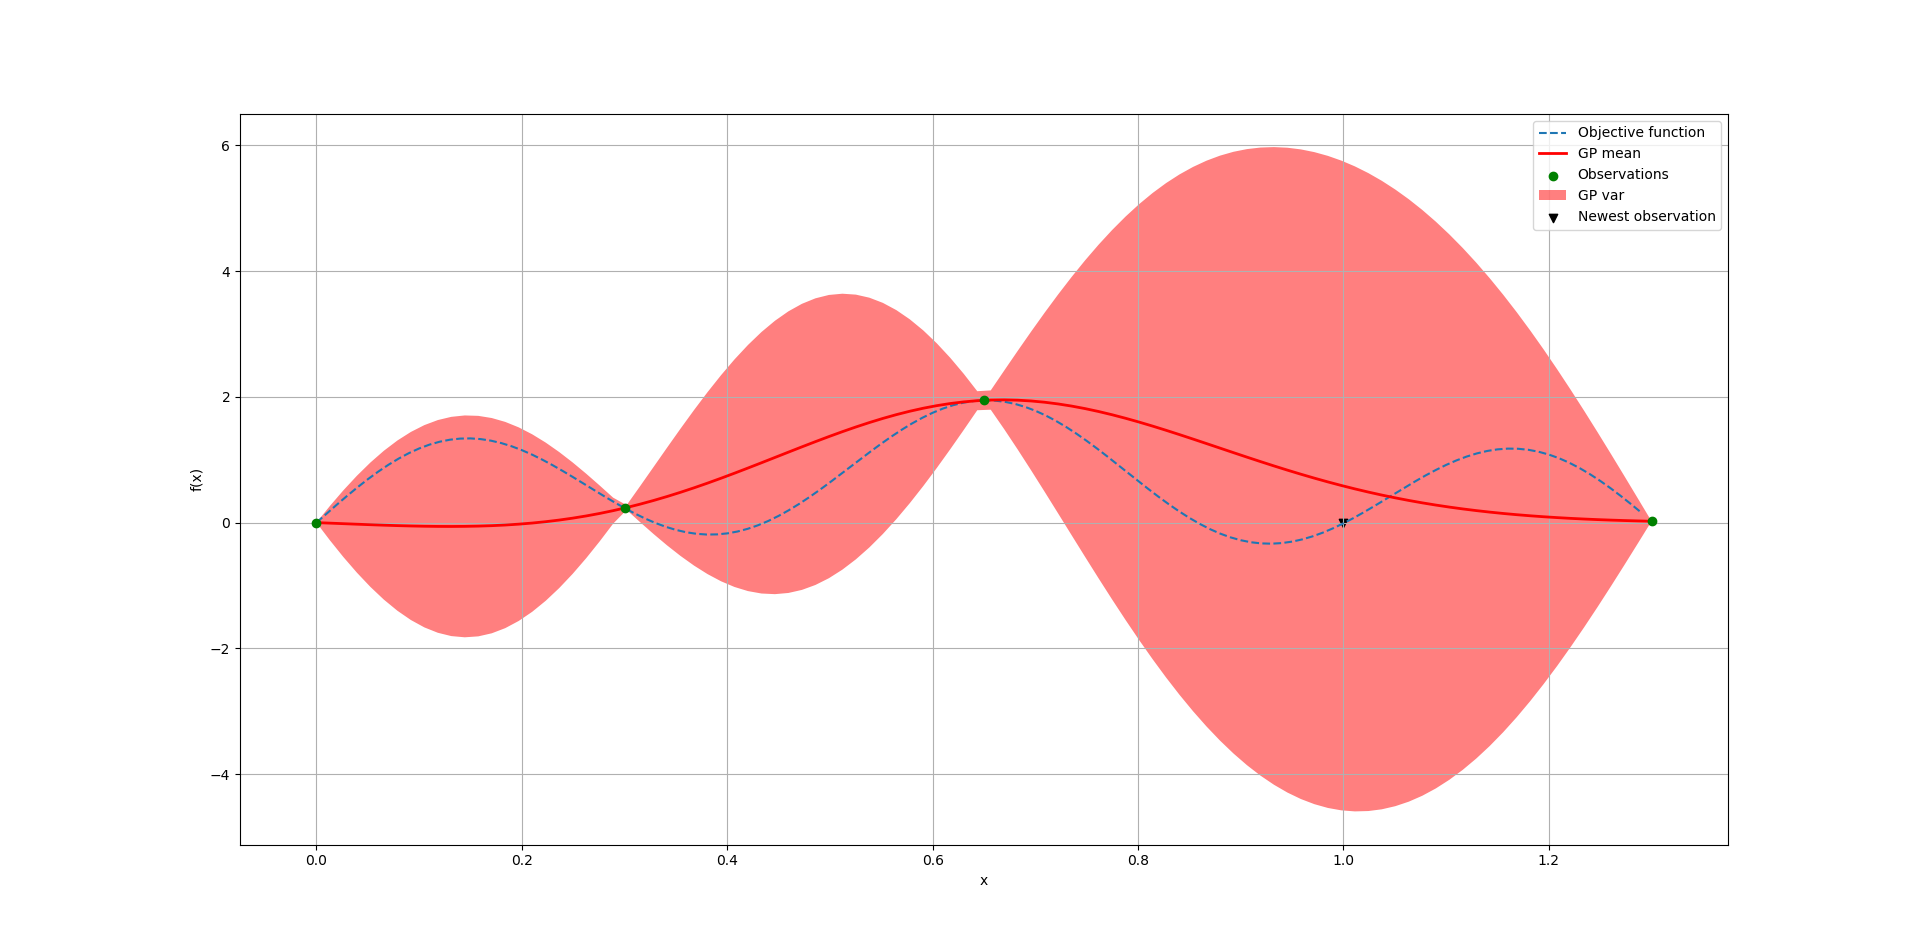
\includegraphics[width=\linewidth]{images/intro_images/BOLoop_2.png}}
%    \only<3>{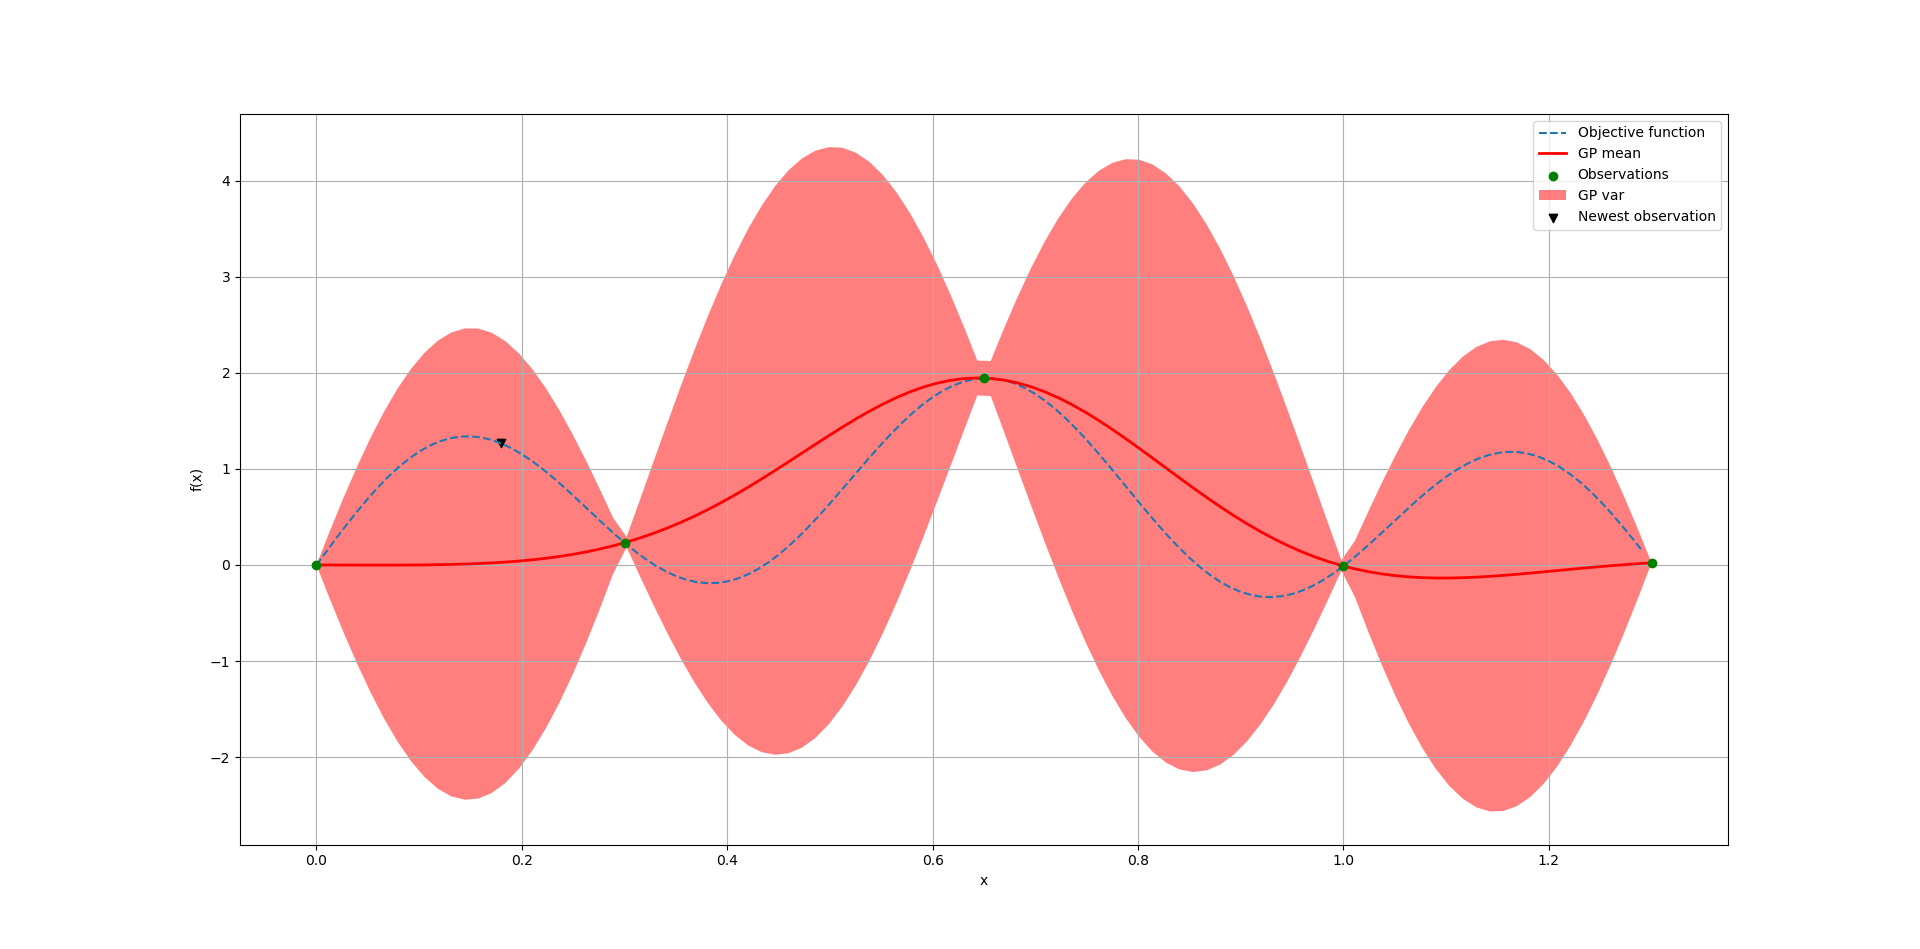
\includegraphics[width=\linewidth]{images/intro_images/BOLoop_3.png}}
%    \only<4>{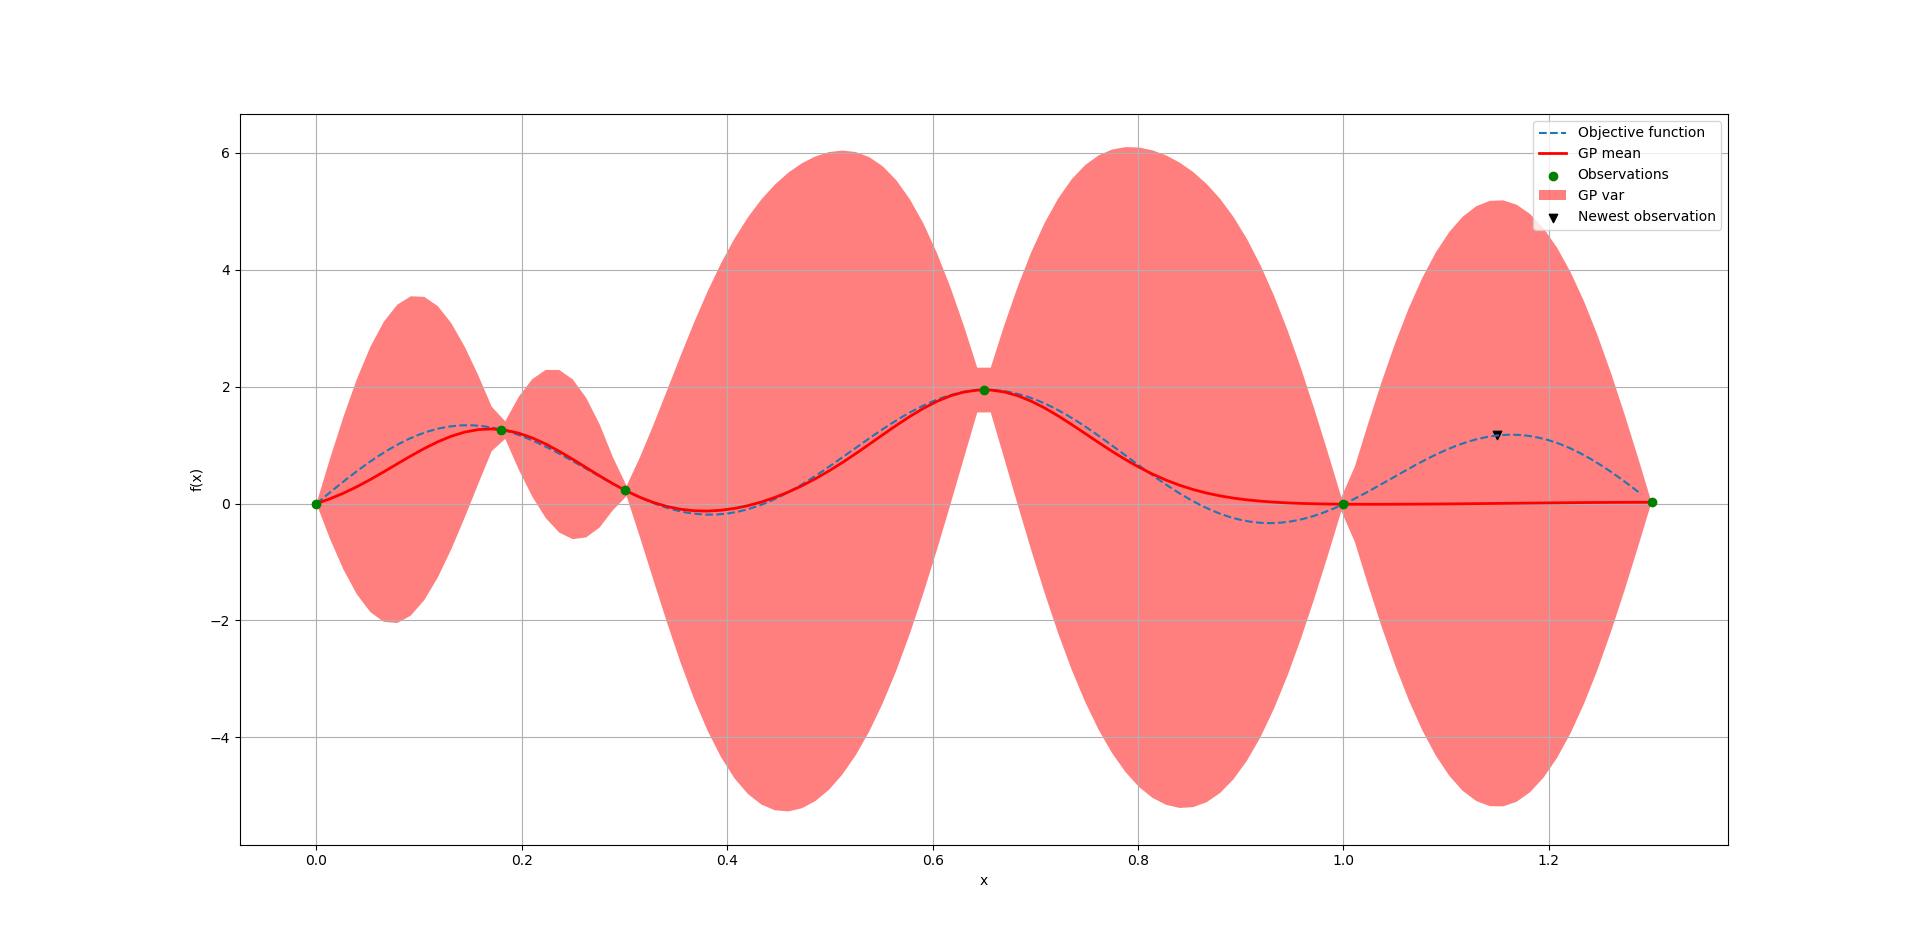
\includegraphics[width=\linewidth]{images/intro_images/BOLoop_4.png}}
%    \only<5>{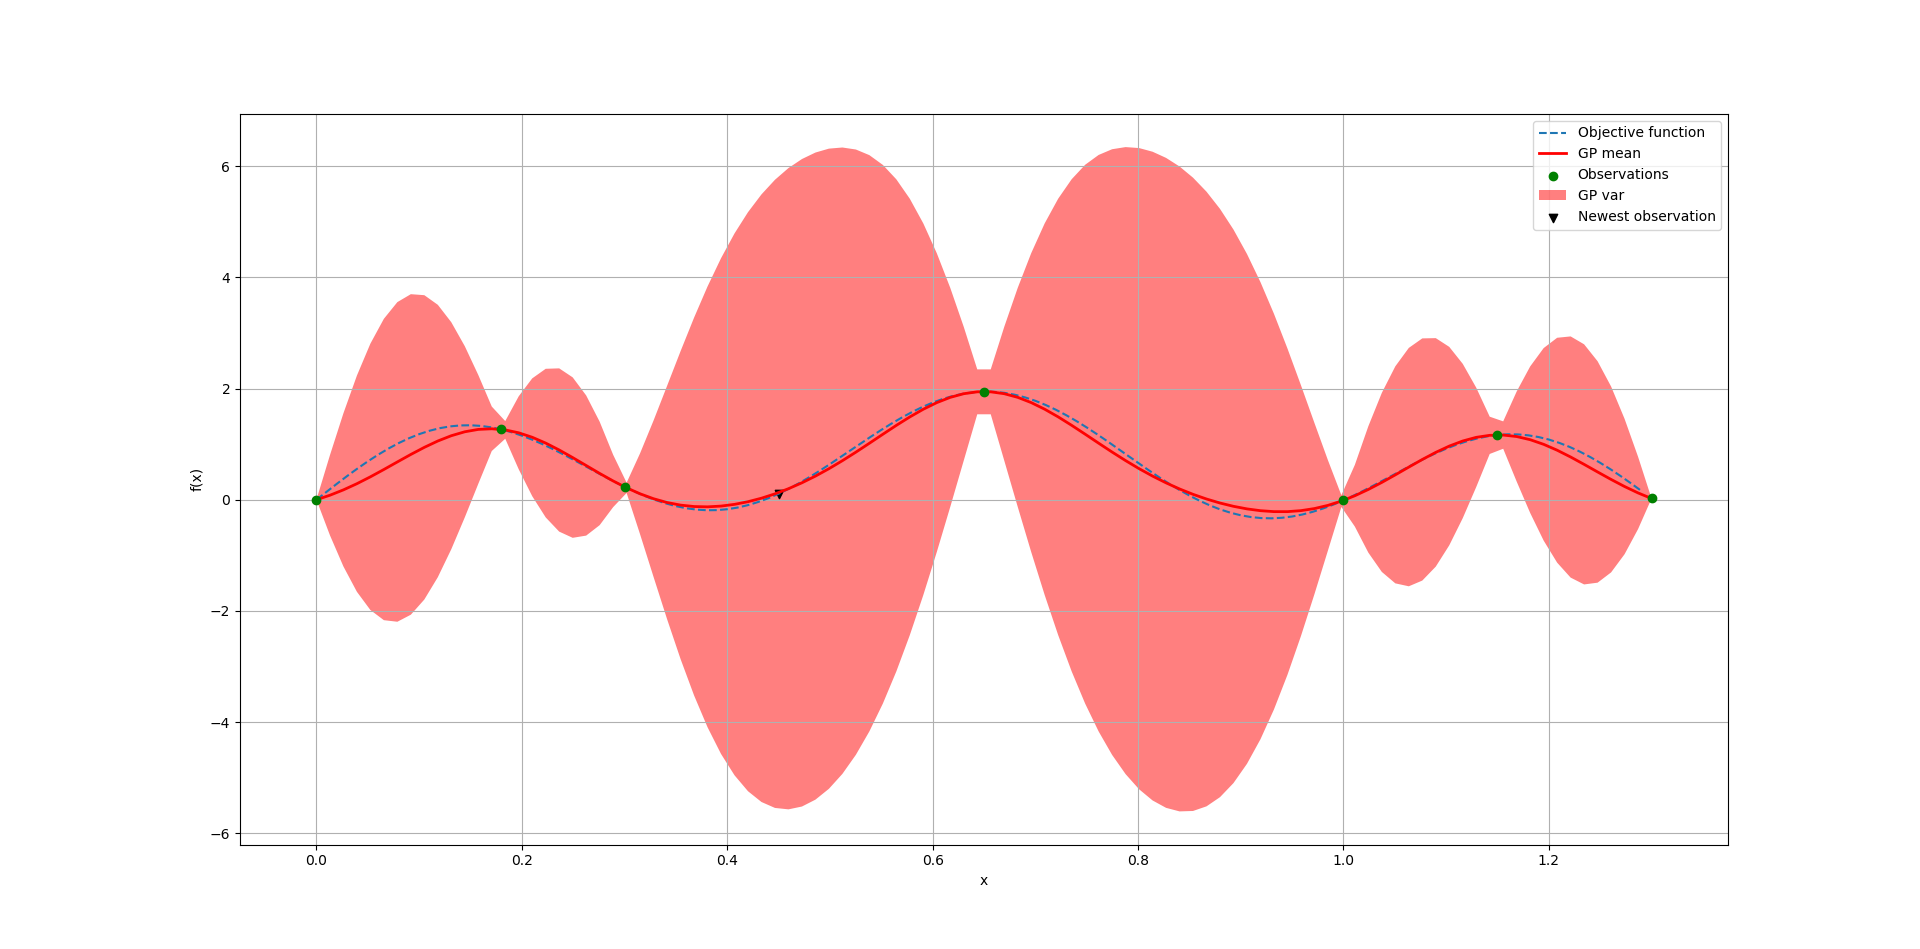
\includegraphics[width=\linewidth]{images/intro_images/BOLoop_5.png}}
%    \only<6>{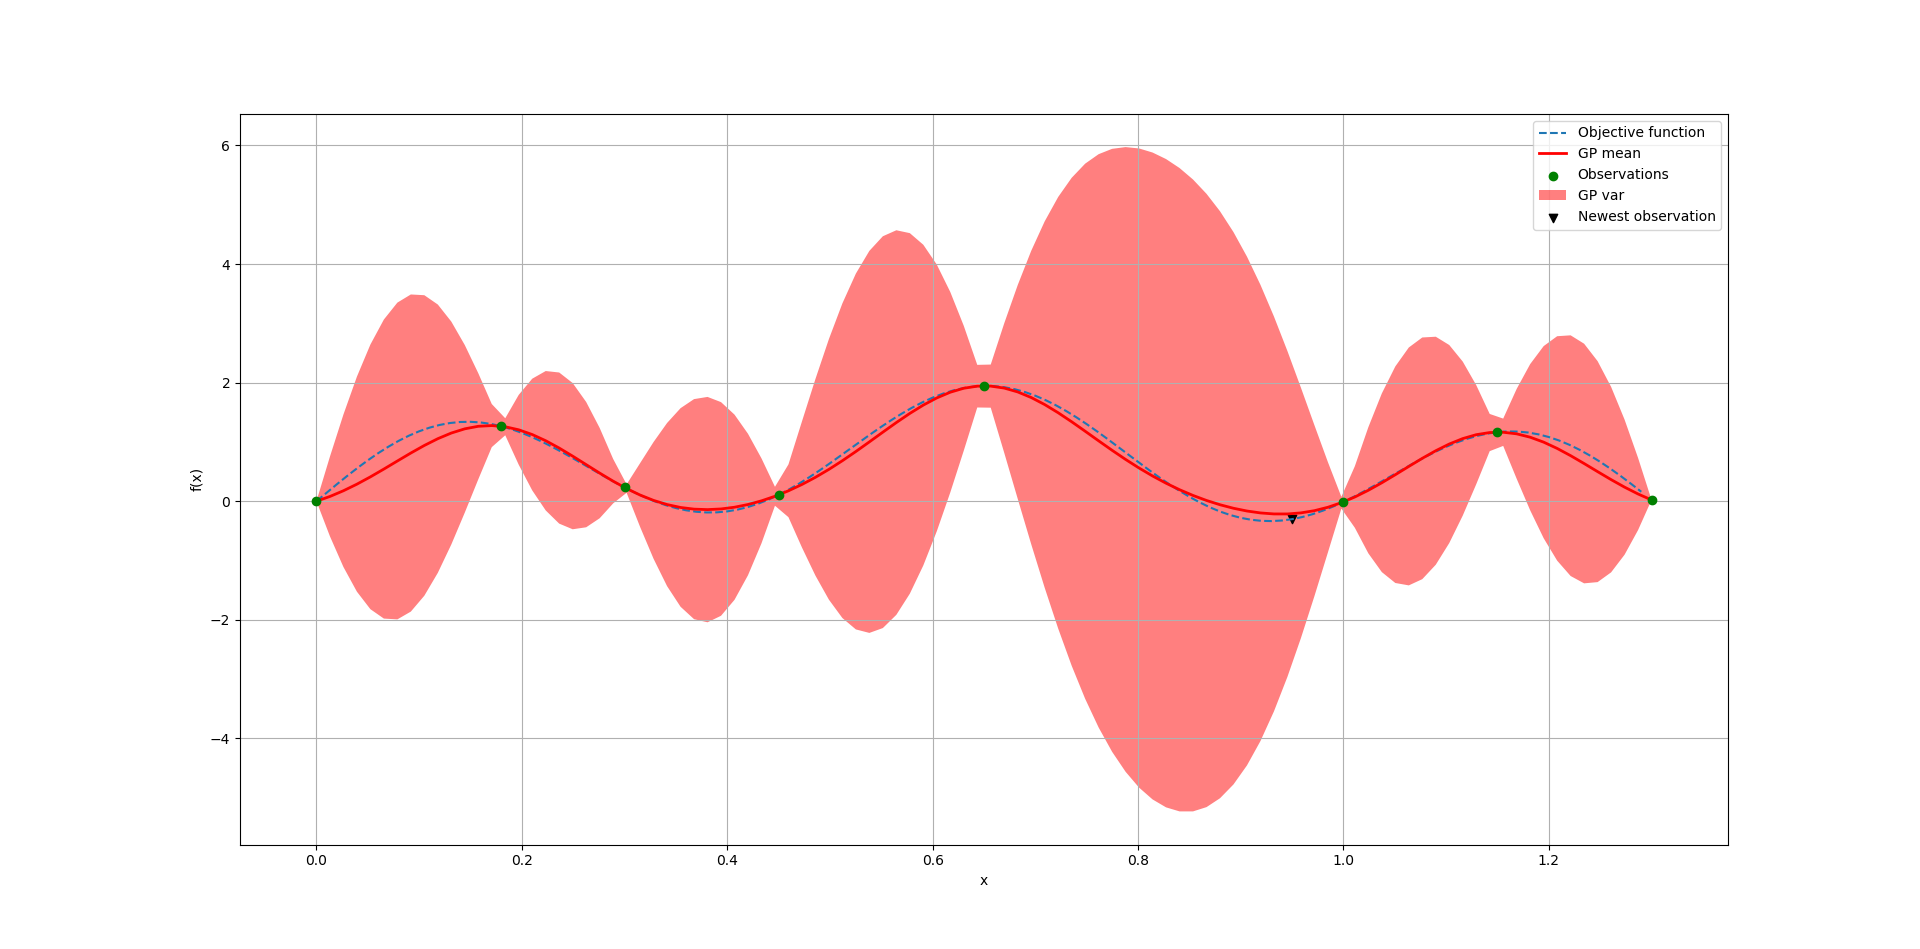
\includegraphics[width=\linewidth]{images/intro_images/BOLoop_6.png}}
%    \only<7>{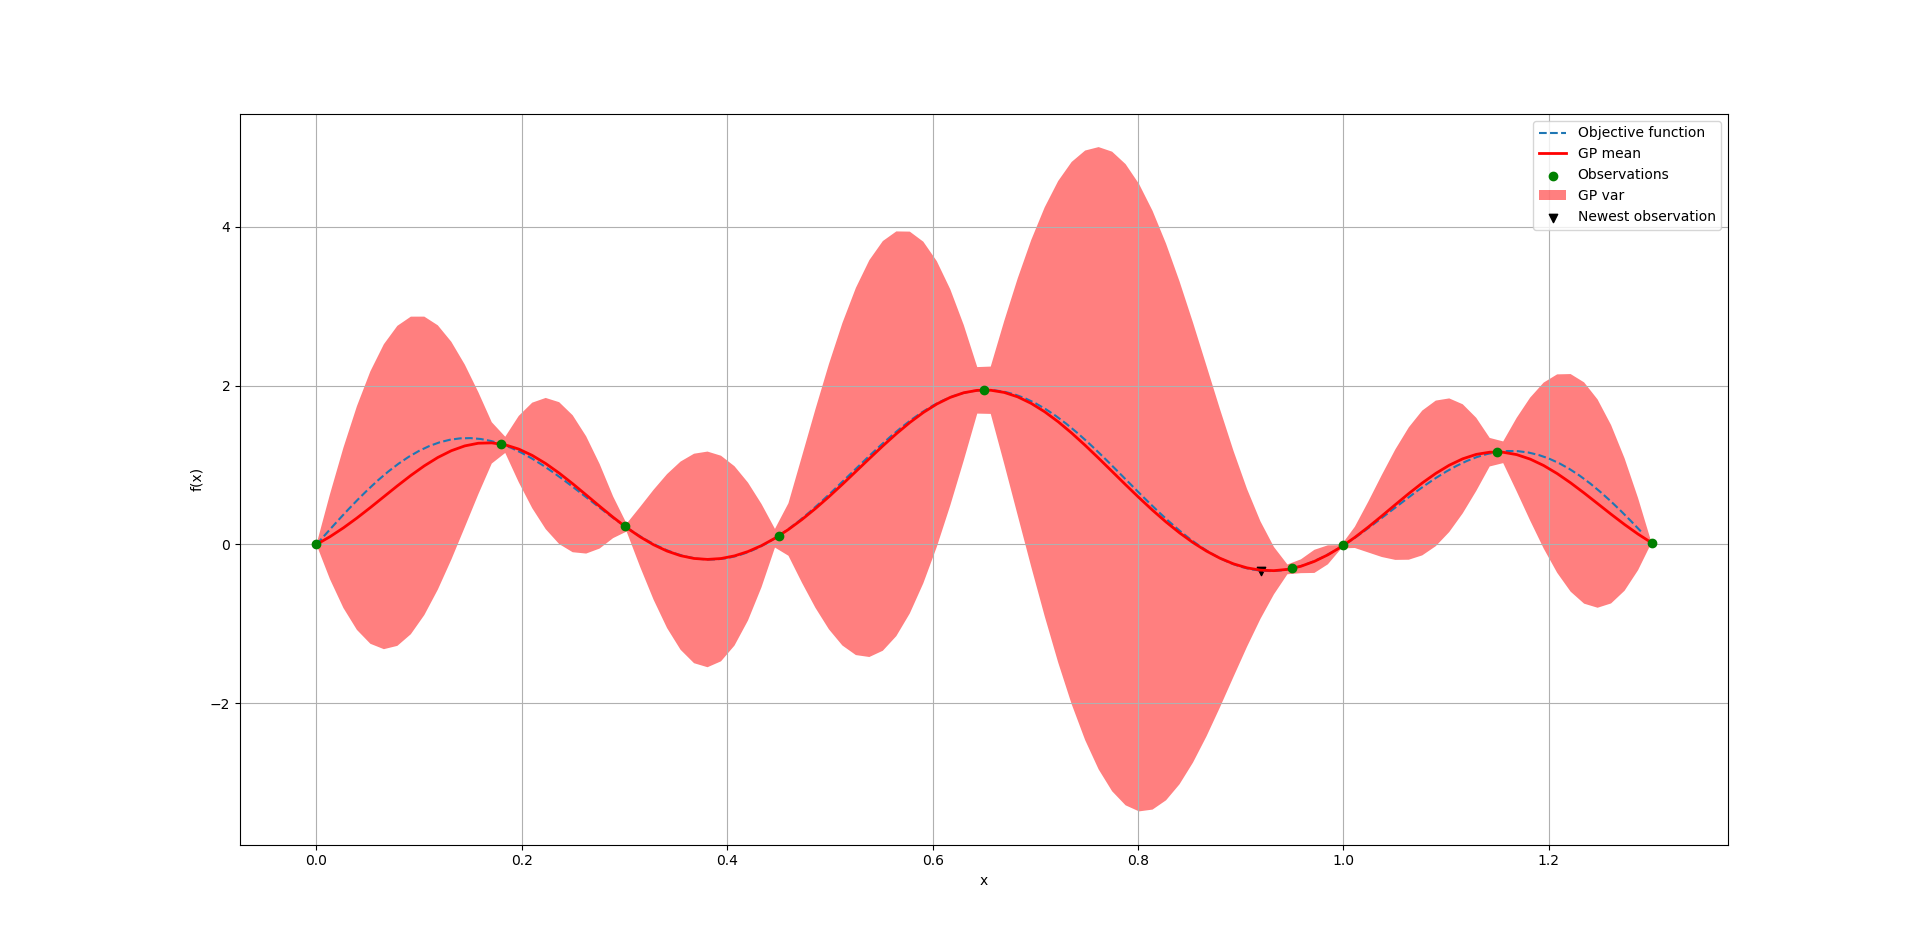
\includegraphics[width=\linewidth]{images/intro_images/BOLoop_7.png}}
%    \only<8>{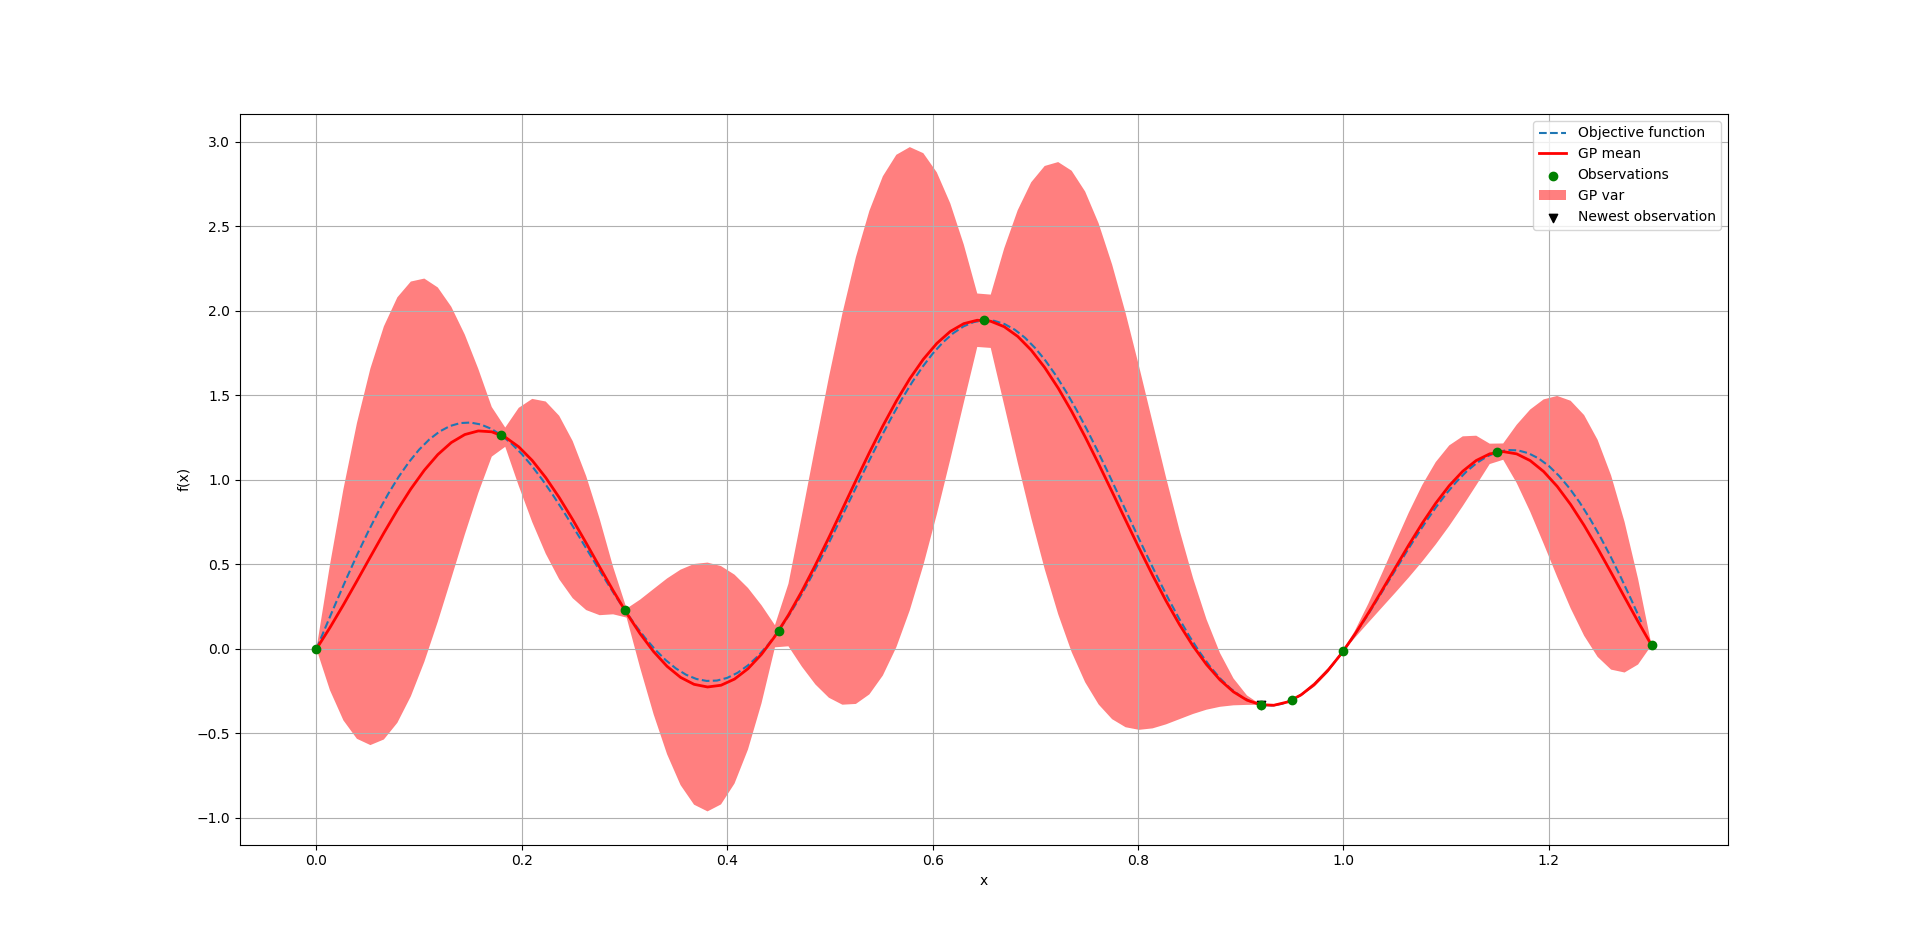
\includegraphics[width=\linewidth]{images/intro_images/BOLoop_8.png}}
%\end{figure}
%\end{frame}
%----------------------------------------------------------------------

\begin{frame}[c]{Bayesian Optimization: Pseudocode}

\begin{center}
\begin{minipage}{0.75\textwidth}
\begin{algorithm}[H]
    %\DontPrintSemicolon
%    \SetAlgoLined
    \setcounter{AlgoLine}{0}
    \SetKwInOut{Require}{Require}
    \SetKwInOut{Result}{Result}
    
    \Require{Search space $\pcs$, 
    		cost function $\cost$, 
    		acquisition function $\acq$, predictive model $\surro$,
    		maximal number of function evaluations $\bobudget$}
    \Result{Best configuration $\finconf$
    (according to $\dataset$ or 
    $\surro$)}
    
	Initialize data $\iter[0]{\dataset}$ with initial observations\;% \leftarrow \varnothing$\; 
	 
    \For{$\bocount=1$ \KwTo $\bobudget$}{
		%\While{$B$ not exhausted} {
		Fit predictive model $\iter[\bocount]{\surro}$ on $\iter[\bocount-1]{\dataset}$\;
		
		Select next query point: $\bonextsample \in \argmax_{\conf \in \pcs} \acq(\conf; \iter[\bocount-1]{\dataset}, \iter[\bocount]{\surro})$\;
		
		Query $\bonextobs$\;
		
		Update data: $\iter[\bocount]{\dataset} \leftarrow \iter[\bocount-1]{\dataset} \cup \{\langle \bonextsample, \bonextobs \rangle \}$\;
	}
	\caption*{BO loop}
\end{algorithm}
\end{minipage}
\end{center}
\end{frame}
%-----------------------------------------------------------------------
\begin{frame}[c]{Bayesian Optimization: Origin of the Name}

\begin{itemize}
    \item Bayesian optimization uses \alert{Bayes' theorem}: 
    	\begin{equation*}
    	    P(A \vert B) = \frac{P(B \vert A) \times  P(A)}{P(B)}
    	    \propto P(B \vert A) \times  P(A)
    	\end{equation*} 
    \item Bayesian optimization uses this to compute a posterior over functions: 
        \begin{equation*}
            P(\func \vert \dataset_{1:\bocount}) \propto P(\dataset_{1:\bocount} \vert \func) \times P(\func), \text{~~~~ where } \dataset_{1:\bocount} = \left \{ \conf_{1:\bocount}, \cost(\conf_{1:\bocount}) \right\}
        \end{equation*} 
\pause
\vspace*{-0.5cm}
    \item Meaning of the individual terms:
        \begin{itemize}
            \item $P(f)$ is the \alert{prior} over functions, which represents our belief about the space of possible objective functions \alert{before} we see any data
            \item $\dataset_{1:\bocount}$ is the \alert{data} (or observations, evidence)
            \item $P(\dataset_{1:\bocount} \vert \func)$ is the likelihood of the data given a function
            \item $P(\func \vert \dataset_{1:\bocount})$ is the \alert{posterior} probability over functions given the data
        \end{itemize}
    \end{itemize}
\end{frame}
%-----------------------------------------------------------------------
\begin{frame}[c]{Bayesian Optimization: Advantages and Disadvantages}

\begin{columns}[T] % align columns
\begin{column}{.48\textwidth}


\begin{block}{Advantages}
\begin{itemize}
  \item Sample efficient 
  \item Can handle noise
  \item Native incorporation of priors 
  \item Does not require gradients 
  \item Theoretical guarantees
\end{itemize}
\end{block}

\end{column}%

\hfill%
\pause 
\begin{column}{.48\textwidth}

\begin{block}{Disadvantages}
\begin{itemize}
  \item Overhead because of model training in each iteration 
  \item Crucially relies on robust surrogate model
  \item Inherently sequential (in its basic form)
\end{itemize}
\end{block}

\end{column}
\end{columns}

\end{frame}
%-----------------------------------------------------------------------
\begin{frame}[c]{Learning Goals of this Lecture}
\framesubtitle{After this lecture, students can ...}

\begin{itemize}
    \item Explain the basics of Bayesian optimization
    \item Derive \alert{simple acquisition functions}
    \item Describe \alert{advanced acquisition functions}
    \item Describe possible \alert{surrogate models} and their pros and cons 
    \item Discuss the \alert{limits of Bayesian optimization} and extensions to tackle these
%    \item Describe the \alert{alternative Bayesian optimization approach of TPE}
    \item Discuss \alert{success stories} of Bayesian optimization
\end{itemize}

\end{frame}

%-----------------------------------------------------------------------
%----------------------------------------------------------------------
%\begin{frame}[c]{Surrogate modelling}
%\framesubtitle{General idea}
%\begin{itemize}
%    \item Use a surrogate model of the expensive function $\cost$ as a cheap-to-evaluate proxy.
%    \begin{itemize}
%        \item Use a probabilistic model with well-calibrated uncertainty predictions.
%    \end{itemize}
%    \pause
%    \item Define a utility function to guide the search for new data points.
%    \pause
%    \item Use the optimization of the utility function as a decision procedure to provide inference on where to evaluate next.
%
%\end{itemize}
%\end{frame}

%-----------------------------------------------------------------------

%\end{document}